\documentclass[a4paper,11pt]{book}
%\documentclass[a4paper,twoside,11pt,titlepage]{book}
\usepackage{listings}
\usepackage[utf8]{inputenc}
\usepackage[spanish]{babel}

% \usepackage[style=list, number=none]{glossary} %
%\usepackage{titlesec}
%\usepackage{pailatino}

\decimalpoint
\usepackage{dcolumn}
\newcolumntype{.}{D{.}{\esperiod}{-1}}
\makeatletter
\addto\shorthandsspanish{\let\esperiod\es@period@code}
\makeatother


%\usepackage[chapter]{algorithm}
\RequirePackage{verbatim}
%\RequirePackage[Glenn]{fncychap}
\usepackage{fancyhdr}
\usepackage{graphicx}
\usepackage{afterpage}

\usepackage{longtable}

\usepackage[pdfborder={000}]{hyperref} %referencia

% ********************************************************************
% Re-usable information
% ********************************************************************
\newcommand{\myTitle}{Mipolla\xspace}
\newcommand{\myDegree}{Grado en ...\xspace}
\newcommand{\myName}{Nombre Apllido1 Apellido2 (alumno)\xspace}
\newcommand{\myProf}{Nombre Apllido1 Apellido2 (tutor1)\xspace}
\newcommand{\myOtherProf}{Nombre Apllido1 Apellido2 (tutor2)\xspace}
%\newcommand{\mySupervisor}{Put name here\xspace}
\newcommand{\myFaculty}{Escuela Técnica Superior de Ingenierías Informática y de
Telecomunicación\xspace}
\newcommand{\myFacultyShort}{E.T.S. de Ingenierías Informática y de
Telecomunicación\xspace}
\newcommand{\myDepartment}{Departamento de ...\xspace}
\newcommand{\myUni}{\protect{Universidad de Granada}\xspace}
\newcommand{\myLocation}{Granada\xspace}
\newcommand{\myTime}{\today\xspace}
\newcommand{\myVersion}{Version 0.1\xspace}


\hypersetup{
pdfauthor = {\myName (email (en) ugr (punto) es)},
pdftitle = {\myTitle},
pdfsubject = {},
pdfkeywords = {palabra_clave1, palabra_clave2, palabra_clave3, ...},
pdfcreator = {LaTeX con el paquete ....},
pdfproducer = {pdflatex}
}

%\hyphenation{}


%\usepackage{doxygen/doxygen}
%\usepackage{pdfpages}
\usepackage{url}
\usepackage{colortbl,longtable}
\usepackage[stable]{footmisc}
%\usepackage{index}

%\makeindex
%\usepackage[style=long, cols=2,border=plain,toc=true,number=none]{glossary}
% \makeglossary

% Definición de comandos que me son tiles:
%\renewcommand{\indexname}{Índice alfabético}
%\renewcommand{\glossaryname}{Glosario}

\pagestyle{fancy}
\fancyhf{}
\fancyhead[LO]{\leftmark}
\fancyhead[RE]{\rightmark}
\fancyhead[RO,LE]{\textbf{\thepage}}
\renewcommand{\chaptermark}[1]{\markboth{\textbf{#1}}{}}
\renewcommand{\sectionmark}[1]{\markright{\textbf{\thesection. #1}}}

\setlength{\headheight}{1.5\headheight}

\newcommand{\HRule}{\rule{\linewidth}{0.5mm}}
%Definimos los tipos teorema, ejemplo y definición podremos usar estos tipos
%simplemente poniendo \begin{teorema} \end{teorema} ...
\newtheorem{teorema}{Teorema}[chapter]
\newtheorem{ejemplo}{Ejemplo}[chapter]
\newtheorem{definicion}{Definición}[chapter]

\definecolor{gray97}{gray}{.97}
\definecolor{gray75}{gray}{.75}
\definecolor{gray45}{gray}{.45}
\definecolor{gray30}{gray}{.94}

\lstset{ frame=Ltb,
     framerule=0.5pt,
     aboveskip=0.5cm,
     framextopmargin=3pt,
     framexbottommargin=3pt,
     framexleftmargin=0.1cm,
     framesep=0pt,
     rulesep=.4pt,
     backgroundcolor=\color{gray97},
     rulesepcolor=\color{black},
     %
     stringstyle=\ttfamily,
     showstringspaces = false,
     basicstyle=\scriptsize\ttfamily,
     commentstyle=\color{gray45},
     keywordstyle=\bfseries,
     %
     numbers=left,
     numbersep=6pt,
     numberstyle=\tiny,
     numberfirstline = false,
     breaklines=true,
   }
 
% minimizar fragmentado de listados
\lstnewenvironment{listing}[1][]
   {\lstset{#1}\pagebreak[0]}{\pagebreak[0]}

\lstdefinestyle{CodigoC}
   {
	basicstyle=\scriptsize,
	frame=single,
	language=C,
	numbers=left
   }
\lstdefinestyle{CodigoC++}
   {
	basicstyle=\small,
	frame=single,
	backgroundcolor=\color{gray30},
	language=C++,
	numbers=left
   }

 
\lstdefinestyle{Consola}
   {basicstyle=\scriptsize\bf\ttfamily,
    backgroundcolor=\color{gray30},
    frame=single,
    numbers=none
   }


\newcommand{\bigrule}{\titlerule[0.5mm]}


%Para conseguir que en las páginas en blanco no ponga cabecerass
\makeatletter
\def\clearpage{%
  \ifvmode
    \ifnum \@dbltopnum =\m@ne
      \ifdim \pagetotal <\topskip
        \hbox{}
      \fi
    \fi
  \fi
  \newpage
  \thispagestyle{empty}
  \write\m@ne{}
  \vbox{}
  \penalty -\@Mi
}
\makeatother

\usepackage{pdfpages}
\begin{document}
\begin{titlepage}
 
 
\newlength{\centeroffset}
\setlength{\centeroffset}{-0.5\oddsidemargin}
\addtolength{\centeroffset}{0.5\evensidemargin}
\thispagestyle{empty}

\noindent\hspace*{\centeroffset}\begin{minipage}{\textwidth}

\centering

\includegraphics[width=0.9\textwidth]{imagenes/logo_ugr.jpg}\\[1.4cm]

\textsc{ \Large TRABAJO FIN DE GRADO\\[0.2cm]}
\textsc{ INGENIERÍA EN INFORMÁTICA}\\[1cm]
% Upper part of the page
% 
% Title
{\Huge\bfseries Despliegue automático de infraestructura + CI/CD \\
}
\noindent\rule[-1ex]{\textwidth}{3pt}\\[3.5ex]
{\large\bfseries Implementación de técnicas DevOps}
\end{minipage}

\vspace{2.5cm}
\noindent\hspace*{\centeroffset}\begin{minipage}{\textwidth}
\centering

\textbf{Autor}\\ {Víctor Moreno Jiménez (alumno)}\\[2.5ex]
\textbf{Directores}\\
{Juan Julián Merelo Guervós}\\[2.5ex]

\includegraphics[width=0.3\textwidth]{imagenes/etsiit_logo.png}\\[0.1cm]
\textsc{Escuela Técnica Superior de Ingenierías Informática y de Telecomunicación}\\
\textsc{---}\\
Granada, Junio de 2020
\end{minipage}
%\addtolength{\textwidth}{\centeroffset}
%\vspace{\stretch{2}}
\end{titlepage}



\chapter*{}
%\thispagestyle{empty}
%\cleardoublepage

%\thispagestyle{empty}

\begin{titlepage}
 
 
\setlength{\centeroffset}{-0.5\oddsidemargin}
\addtolength{\centeroffset}{0.5\evensidemargin}
\thispagestyle{empty}

\noindent\hspace*{\centeroffset}\begin{minipage}{\textwidth}

\centering
%
\includegraphics[width=0.9\textwidth]{imagenes/logo_ugr.jpg}\\[1.4cm]

%\textsc{ \Large PROYECTO FIN DE CARRERA\\[0.2cm]}
%\textsc{ INGENIERÍA EN INFORMÁTICA}\\[1cm]
% Upper part of the page
% 

 \vspace{3.3cm}

%si el proyecto tiene logo poner aquí
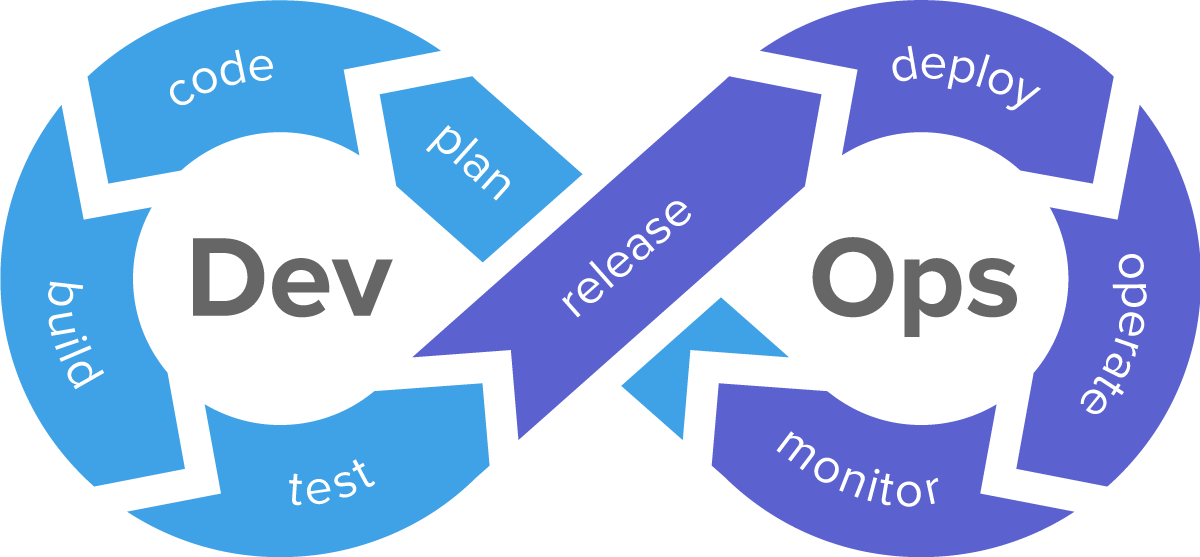
\includegraphics[width=0.9\textwidth]{imagenes/logo4.png}\\[1.4cm]
 \vspace{0.5cm}

% Title

{\Huge\bfseries Despliegue automático de infraestructura + CI/CD\\
}
\noindent\rule[-1ex]{\textwidth}{3pt}\\[3.5ex]
{\large\bfseries Implementación de técnicas DevOps \\[4cm]}
\end{minipage}

\vspace{2.5cm}
\noindent\hspace*{\centeroffset}\begin{minipage}{\textwidth}
\centering

\textbf{Autor}\\ {Víctor Moreno Jiménez}\\[2.5ex]
\textbf{Directores}\\
Juan Julián Melero Guervós \\[2cm]
%
\includegraphics[width=0.15\textwidth]{imagenes/tstc.png}\\[0.1cm]
%\textsc{Departamento de Teoría de la Señal, Telemática y Comunicaciones}\\
%\textsc{---}\\
%Granada, mes de 201
\end{minipage}
%\addtolength{\textwidth}{\centeroffset}
\vspace{\stretch{2}}

 
\end{titlepage}





\cleardoublepage
\thispagestyle{empty}

\begin{center}
{\large\bfseries  Despliegue automático de infraestructura + CI/CD: Implementación de técnicas DevOps}\\
\end{center}
\begin{center}
Víctor Moreno Jiménez\\
\end{center}

%\vspace{0.7cm}
\noindent{\textbf{Palabras clave}: DevOps, IaC (Infraestructure as Code), CI (Continous Integration), CD (Continous Delivery)}\\

\vspace{0.7cm}
\noindent{\textbf{Resumen}}\\

El objetivo de este TFG es implementar las técnicas actuales conocidas como DevOps en una empresa con limitados recursos. \bigskip

En concreto se va a automatizar todo el proceso de despliegue de infraestructura (IaC) y se van a aplicar los principios de integración contínua y entrega contínua propios de la filosofía DevOps en todo el ciclo de desarrollo de los productos de la empresa. \bigskip

La finalidad de esto es poder disponer de una infraestructura sólida y facilmente recreable en caso de catástrofe o ampliación del cluster. Desde el punto de vista de los desarrolladores de la empresa, podrán tener a su disposición y bajo demanda, un entorno de desarrollo mediante ficheros de configuración sin depender directamente del departamento de sistemas. \bigskip

\cleardoublepage


\thispagestyle{empty}


\begin{center}
{\large\bfseries Automatic deployment of infrastructure + CI / CD: Implementation of DevOps techniques}\\
\end{center}
\begin{center}
Víctor Moreno Jiménez\\
\end{center}

%\vspace{0.7cm}
\noindent{\textbf{Keywords}: DevOps, IaC (Infraestructure as Code), CI (Continous Integration), CD (Continous Delivery)}\\

\vspace{0.7cm}
\noindent{\textbf{Abstract}}\\

The main goal of this project is to apply known DevOps techniques in a company with limited resources.\bigskip

The entire company infraestructure will be automated using some orchestration tools via configuration files (Infrastructure as Code). DevOps philosphy will be applied throughout the development cycle of the company's products. \bigskip

The purpose of this is to be able to have a solid and easily deployable infrastructure. From the point of view of the company's developers, they will have the hability to create development infrastructures on demand without depending directly on the systems department \bigskip



\chapter*{}
\thispagestyle{empty}

\noindent\rule[-1ex]{\textwidth}{2pt}\\[4.5ex]

Yo, \textbf{Victor Moreno Jiménez}, alumno de la titulación Ingeniería Informática de la \textbf{Escuela Técnica Superior
de Ingenierías Informática y de Telecomunicación de la Universidad de Granada}, con DNI XXXXXXXXX, autorizo la
ubicación de la siguiente copia de mi Trabajo Fin de Grado en la biblioteca del centro para que pueda ser
consultada por las personas que lo deseen.

\vspace{6cm}

\noindent Fdo: Víctor Moreno Jiménez

\vspace{2cm}

\begin{flushright}
Granada a 31 de Julio de 2020.
\end{flushright}


\chapter*{}
\thispagestyle{empty}

\noindent\rule[-1ex]{\textwidth}{2pt}\\[4.5ex]

D. \textbf{Juan Julián Merelo Guervós}, Profesor del Área de XXXX del Departamento YYYY de la Universidad de Granada.


\vspace{0.5cm}

\textbf{Informan:}

\vspace{0.5cm}

Que el presente trabajo, titulado \textit{\textbf{Automatic deployment of infrastructure + CI / CD: Implementation of DevOps}},
ha sido realizado bajo su supervisión por \textbf{Víctor Moreno Jiménez}, y autorizamos la defensa de dicho trabajo ante el tribunal
que corresponda.

\vspace{0.5cm}

Y para que conste, expiden y firman el presente informe en Granada a 25 de Agosto de 2020.

\vspace{1cm}

\textbf{Los directores:}

\vspace{5cm}
\noindent Fdo: Juan Julián Merelo Guervós



\chapter*{Agradecimientos}
\thispagestyle{empty}

       \vspace{1cm}


Para toda la gente maravillosa que me he cruzado en estos 4 años de carrera. No habría sido lo mismo sin vosotros... Gracias


\frontmatter
\tableofcontents
\listoffigures
\listoftables
%
\mainmatter
\setlength{\parskip}{5pt}

\chapter {Introducción}
\label{capitulo1}
	\begin{paragraph}
		Actualmente trabajo como administrador de sistemas en una empresa de desarrollo de aplicaciones web. Este proyecto es una colaboración con la empresa con el fin de mejorar técnicamente toda la infraestructura necesaria para desarrollar la actividad de la empresa. Principalmente una mejora en los tiempos de creación/replicación de infraestructura y en los cauces de desarrollo de software. A continuación se detalla el alcance del proyecto así como una definición específica del problema que se pretende resolver.
	\end{paragraph}

\section{Accesibilidad del proyecto}
\begin{text}
	Este proyecto ha sido desarrollado bajo la licencia \textbf{GNU General Public License v3.0} y es de carácter público. Se puede acceder a este a través de GitHub en el siguiente \href{https://github.com/VictorMorenoJimenez/tfg2020}{enlace}. Cualquiera puede contribuir al código a través de un pull request. También forma parte de los \href{https://github.com/JJ/TF-libres-UGR}{trabajos liberados} de la UGR.
\end{text}
\section{Definición del problema}
	\begin{text}
		Actualmente la empresa para la que trabajo dispone de una infraestructura desplegada en un proveedor de servidores bare metal, esta infraestructura se ha ido creando con el tiempo, añadiendo servicios y haciendo las modificaciones pertinentes de forma manual. \\
		Dicha infraestructura es la responsable de alojar todos los servicios que ofrecen a los clientes y se utiliza también para el desarrollo de nuevo software. Los desarrolladores utilizan máquinas virtuales para simular entornos de producción donde desplegar las aplicaciones en fase de pruebas antes de hacer un despliegue definitivo en producción. \\
		Esto plantea varios problemas:
		\begin{itemize}
			\item Infraestructura configurada manualmente, imposible de replicar rápidamente.
			\item Configuración de los distintos servicios manual, imposible de replicar rápidamente. 
			\item Difícil conocer el estado actual de los distintos servicios desplegados. 
			\item Imposible replicar la infraestructura en tiempos asequibles ante fallo total.
			\item Los desarrolladores dependen del equipo de sistemas para incorporar cambios en aplicaciones en pruebas.
			\item Ralentización de los procesos de desarrollo de software debido a la dependencia del equipo de sistemas.
		\end{itemize}
	\end{text}

\section{Objetivos}
\label{objetivos_primarios}
\begin{text}
	Una vez identificados los problemas podemos definir una serie de objetivos a alcanzar para solucionarlos. Este proyecto pretende lograr:
	\begin{itemize}
		\item \textbf{Objetivo 1}. Asegurar unos tiempos bajos en la creación de infraestructura para proveer servicios.
		\item \textbf{Objetivo 2}. Replicar la infraestructura asegurando bajos tiempos de creación.
		\item \textbf{Objetivo 3}. Crear servicios necesarios para una empresa de aplicaciones web asegurando bajos tiempos de creación.
		\item \textbf{Objetivo 4}. Replicar cualquier servicio alojado en la infraestructura de forma rápida.
		\item \textbf{Objetivo 5}. Crear cauces rápidos y seguros para la creación de nuevo software.
	\end{itemize}
\end{text}

\clearpage 

\section{Conceptos básicos}
		\begin{text}
			A continuación se van a describir uno a uno, los conceptos básicos para entender este proyecto. Son conceptos claves sin los cuales un lector no experto en el tema a tratar, no comprenderá ni el problema ni la solución adoptada para el problema.
		\end{text}
	\subsection{DevOps}
		\begin{text}
			El término DevOps es una fusión de las dos palabras Desarrollo y Operaciones. DevOps es una filosofía, una forma de abordar el desarrollo de software. El objetivo de DevOps es fusionar los departamentos desarrollo y operaciones de forma que sea más fácil y rápida la creación de software. La siguiente imagen define el término:
			
			\begin{figure}[!hbt]
				\centering
				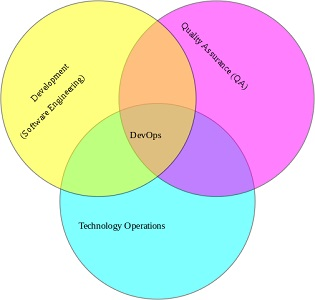
\includegraphics[scale=0.75]{imagenes/Introduccion/Conceptos_Basicos/devops.jpg}
				\caption[¿Qué es DevOps?]{¿Qué es DevOps? \cite{WhatIsDe1:online}}
				\label{termino_devops}
			\end{figure}
		\end{text}
	
	\clearpage 
	
	\subsection{Integración Continua (CI)}
		\begin{text}
			La Integración Continua o CI para abreviar, es uno de los pilares de la filosofía DevOps. La integración continua se basa en hacer integraciones automáticas de un proyecto lo más a menudo posible para poder detectar fallos rápidamente. Consta de dos partes: compilación y ejecución de test de un proyecto.
			
			
			\begin{figure}[!hbt]
				\centering
				\includegraphics[scale=0.45]{imagenes/Introduccion/Conceptos_Basicos/ci.png}
				\caption[Integración Continua]{Integración Continua \cite{Alcanzan90:online} }
				\label{integracion_continua} 
			\end{figure}
		\end{text}
	\subsection{Despliegue continuo (CD)}
		\begin{text}
			El despliegue continuo o CD por sus siglas en inglés 'continous delivery' complementa a la integración continua desplegando el proyecto software en los servidores, una vez ha pasado el proceso de la integración continua. Gracias a 'continous delivery' podemos garantizar entregas rápidas y seguras de software.
			
			\begin{figure}[!hbt]
				\centering
				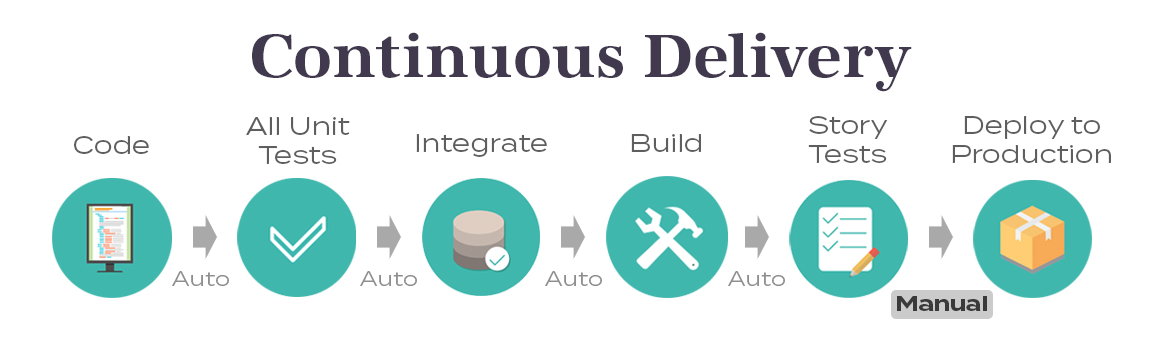
\includegraphics[scale=0.35]{imagenes/Introduccion/Conceptos_Basicos/CD.png}
				\caption[Despliegue Continuo]{Despliegue Continuo \cite{continuo84:online}}
				\label{despligue_continuo} 
			\end{figure}
		\end{text}
	\subsection{Infraestructura como Código (IaaC)}
		\begin{text}
			La infraestructura como código pretende tratar los servidores y toda la infraestructura alrededor de una organización como un software de programación. De este modo, la infraestructura está escrita en ficheros de configuración y es fácilmente replicable y testeable. Este concepto al igual que los dos anteriores está íntimamente ligado con el término DevOps, ya que es uno de los primeros pasos a adoptar. IaaC pretende difuminar la línea entre el código que ejecutan las aplicaciones y el código que configura la infraestructura. Acerca a los desarrolladores al equipo de operaciones o administradores de sistemas. \\
			De esta manera no únicamente se testea el software antes de ser lanzado, si no también la infraestructura. A continuación se muestra como sería el cauce de trabajo siguiendo los principios de IaaC.
			
			\begin{figure}[!hbt]
				\centering
				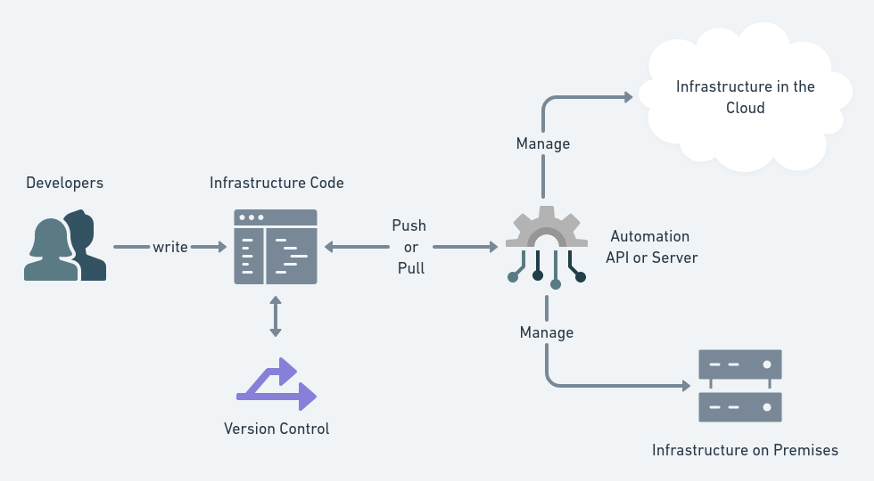
\includegraphics[scale=0.75]{imagenes/Introduccion/Conceptos_Basicos/IaaC.png}
				\caption[Infraestructura como Código]{Infraestructura como Código \cite{WhatIsIaaC:online}}
				\label{infraestructura_como_codigo} 
			\end{figure}
		\end{text}
	
\section{Solución propuesta}
\begin{text}
	Este proyecto se ha creado para cumplir con los objetivos descritos en la sección ``\nameref{objetivos_primarios}''. A continuación se define a grandes rasgos la solución propuesta que se irá justificando y ampliando a lo largo del documento. \\
	\begin{itemize}
		\item \textbf{Objetivo 1: Asegurar unos tiempos bajos en la creación de infraestructura para proveer servicios}. \\ Aplicando la filosofía DevOps a la infraestructura. Se tratará la infraestructura como si fuese un proyecto software, es decir, la infraestructura será codificada bajo ficheros de configuración y estos estarán alojados en algún sistema de control de versiones.
		\item \textbf{Objetivo 1.1: Infraestructura segura frente a ataques}. \\ Para garantizar la seguridad de la infraestructura, se desplegarán firewalls redundantes. Estos firewalls serán tratados como servicios y entran dentro de las especificaciones del objetivo 3.
		\item \textbf{Objetivo 2: Replicar la infraestructura asegurando bajos tiempos de creación.} \\
		Si se consigue objetivo 1, es decir, tener la infraestructura codificada en ficheros de configuración con alguna herramienta de automatización, esta será fácilmente replicable. Si se cumple el objetivo 1, se cumplirá el objetivo 2.
		\item \textbf{Objetivo 3: Crear y desplegar servicios necesarios para una empresa de aplicaciones web asegurando bajos tiempos de creación.} \\
		Una vez cumplidos objetivos 1 y 2, y con una infraestructura base desplegada, será necesario desplegar los servicios que una empresa, dedicada al desarrollo de aplicaciones web requiere. Servicios como servidores web, servicios de orquestación de contenedores, gestor de paso de mensajes... Para garantizar que estos servicios se pueden crear y desplegar en tiempos eficientes, será necesario utilizar herramientas de automatización, de manera que, mediante ficheros de configuración lanzados en la infraestructura, logramos el despliegue de todos los servicios necesarios.
		\item \textbf{Objetivo 4: Crear cauces rápidos y seguros para la creación de nuevo software.} \\
		Para cumplir con este objetivo se va a instalar un servicio en la infraestructura que permita la creación de dichos cauces. Se aplicarán técnicas para garantizar los despliegues automáticos y la creación de entornos de pruebas para probar las aplicaciones. La seguridad está garantizada ya que todo sucede en un entorno seguro gracias al subobjetivo 1.1, y en una red LAN a la cual únicamente tienen acceso los administradores.
	\end{itemize}
\end{text}


%
%\chapter {Análisis del sistema}

%\section{Definición del problema}
%\begin{text}
%	Hoy en día, aún hay muchas compañías que siguen teniendo dos equipos diferenciados dentro el departamento de IT. Sistemas o Operaciones y Desarrolladores. Ya hemos visto en la introducción que esto a la larga causa problemas y no es la forma más rápida y eficiente de desarrollar software. \\
%	Trabajo como Administrador de Sistemas en una empresa pequeña y continuamente aparecen problemas. Es por eso que se ha decidido adoptar un enfoque DevOps par el desarrollo del software. En este cambio están implicados ambos departamentos ya que es responsabilidad de ambos que los cauces de desarrollo y despliegue funcionen correctamente. \\
%	En mi compañía la Infraestructura donde se alojan los proyectos, se configura manualmente haciendo prácticamente imposible una replicación de ésta en caso de que sea necesario. También las subidas de proyectos y ejecución de tests no están automatizados y cada desarrollador se encarga de ejecutar los tests en local. Ésto implica discrepancias varias entre el equipo de operaciones y el de desarrolladores. Es por esto que se hace necesario la adopción de técnicas DevOps como IaaC, CI y CD en la empresa.
%\end{text}
%\section{Que se pretende resolver}
%		\begin{itemize}
%			\item Todos los problemas que involucra la configuración manual de infraestructura.
%			\item Ralentización de desarrollo de software, al no tener los cauces automatizados.
%		\end{itemize}
\section{Casuísticas que se dan y como se resuelve cada una}
		\begin{itemize}
			\item \textbf{Problema 1}: \textit{Recreación ante fallo total o réplica de infraestructura}. Ante un fallo total de la infraestructura o replicación para propósitos de testing, con los sistemas actuales sería imposible, ya que dada la configuración manual de cada uno de los servidores, sería imposible replicar al 100\% el estado de los servidores. 
			
			\item  \textbf {Solución 1}: Al adoptar IaaC, la infraestructura estará codificada en ficheros de configuración bajo control de versiones. Pudiendo recrear la infraestructura bajo demanda en cualquier momento y asegurándonos de que sea la misma al 100%.
			
			\item \textbf{Problema 2}: \textit{Diferencias entre servidor de desarrollo y producción}. Al desarrollar en local, los desarrolladores no tienen una réplica de los servidores de producción para poder probar sus cambios. Esto hace que haya discrepancias entre Sistemas y desarrolladores puesto que puede funcionar en local con una configuración dada pero no en producción. 
			
			\item \textbf {Solución 2}: Al estar la infraestructura de cada aplicación codificada y bajo control de versiones, será sencillo replicar el entorno de producción en un entorno test para el desarrollo de aplicaciones.
			
			\item \textbf{Problema 3}: \textit{Petición de subidas a producción}. Al no existir cauces de integración o despliegue, no se tiene un conocimiento exacto de qué comportamiento va a tener la aplicación en producción. Esto y la necesidad de hacer peticiones al equipo de sistemas para subir nuevas versiones a producción ralentizan el desarrollo del software.
			
			\item \textbf{Solución 3:} Al tener el desarrollador un servidor réplica de producción para desplegar las aplicaciones, sabe perfectamente el comportamiento que va a tener en producción, puesto que son entornos idénticos. Esto y los cauces CI-CD solucionan el problema.
			
			\item \textbf{Problema 4}: \textit{Desconocimiento estado infraestructura o servicios}. Al configurarse los servidores de forma manual, parche tras parche, es imposible conocer en qué estado se encuentra la infraestructura. También dificulta la replicación de esta para procesos de pruebas.
			
			\item \textbf{Solución 4:} Misma solución que Problema 1. Al adoptar IaaC, la infraestructura estará codificada en ficheros de configuración bajo control de versiones. Esto facilita saber qué paquetes hay instalados en el sistema y qué configuración se ha desplegado para cada servicio.	
		\end{itemize}

\section{Metodología de desarrollo}
\begin{text}
	Todo proyecto software debe tener una organización y unas etapas de desarrollo bien definidas. En esta sección se pretende explicar la metodología de desarrollo elegida para realizar este proyecto. \\
	Se ha tratado este proyecto como cualquier otro proyecto software. Para la organización y el control de versiones se ha elegido Github, un software basado en git originalmente creado para el control de versiones. Actualmente, GitHub ofrece múltiples servicios, como almacenamiento, gestión de paneles de trabajo, registry, integración con múltiples tecnologías... \\
	En cuanto a la metodología de desarrollo, se ha optado por un desarrollo basado en Milestones. Cada Milestone está compuesto por Issues y estos están etiquetados y asignados a personas. A continuación se explican con mayor detalle estos conceptos.
\end{text}

\subsection{Milestones}
\label{milestones}
\begin{text}
	Los Milestones o Hitos en castellano, corresponden con estados finales deseados de la aplicación. Sabiendo esto, podríamos crear un Milestone por ejemplo: "Servidores configurados a través de ficheros de configuración Ansible". Esto será un estado final deseado para nuestra aplicación o proyecto. Para que un hito quede totalmente realizado, deben estar completos todos los issues marcados como esenciales para el hito. Un hito está compuesto por issues. A continuación se muestran algunos milestones creados en este proyecto, en el panel de administración GitHub.
	
	\begin{figure}[!hbt]
		\centering
		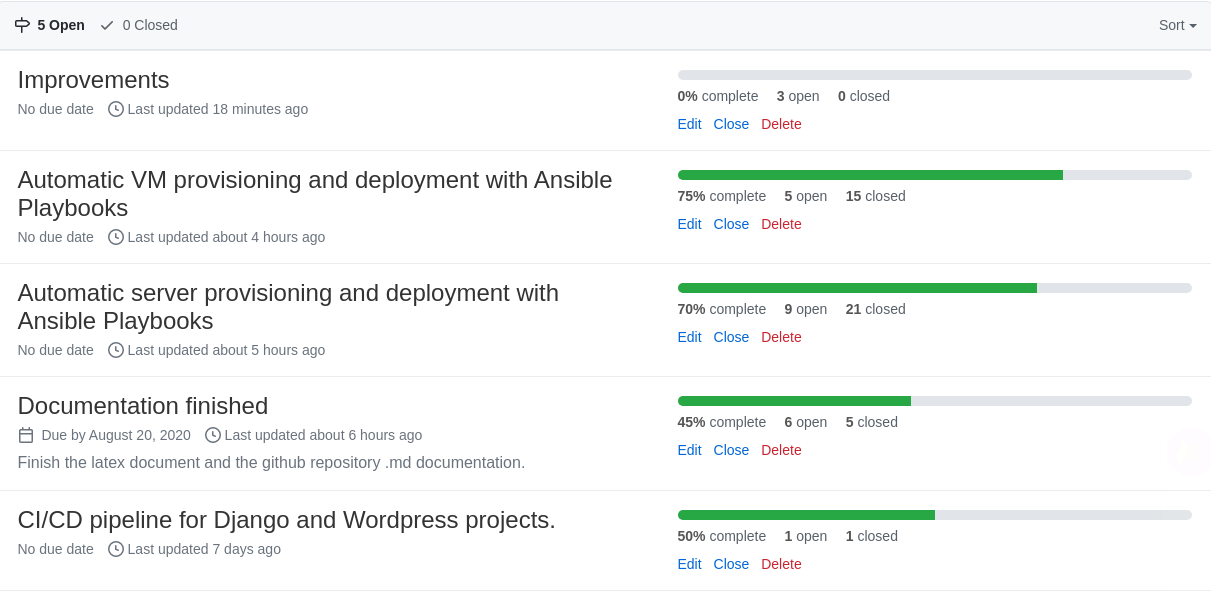
\includegraphics[scale=0.37]{imagenes/Analisis/milestones.png}
		\caption[GitHub milestones]{GitHub milestones}
		\label{github_milestones}
	\end{figure}
\end{text}
\subsection{Issues}
\begin{text}
	Como ya hemos visto, los issues forman parte de los hitos. Es una forma de desgranar el problema. Siguiendo el ejemplo anterior, si tenemos un hito: "Servidores configurados a través de ficheros de configuración Ansible", podemos desgranar el siguiente en distintos issues, que serían tareas más sencillas que hay que realizar para completar el hito. Por ejemplo, algunos issues serían: 
	\begin{itemize}
		\item Crear estructura directorios Ansible.
		\item Instalar paquetes en servidor a través de ficheros de configuración Ansible. \textbf{Core}
		\item Configurar interfaces de red a través de ficheros de configuración Ansible. \textbf{Core}
		\item Instalar ISO en servidor a través de ficheros de configuración Ansible. \textbf{Core}
		\item Instalar certificados SSL a través de ficheros de configuración Ansible. \textbf{Mejora}
	\end{itemize}
	
	Y así seguiríamos creando issues según creamos que van a ser necesarios para completar el hito en cuestión. \\
	En la sección  \nameref{milestones} hemos hablado que los issues tienen etiquetas. En la lista anterior por ejemplo, únicamente tenemos dos etiquetas que nos indican en este caso si son issues imprescindibles para el hito o simplemente mejoras. Gracias a estas etiquetas, podemos distinguir entre distintos tipos de issues y asignar mayor o menos prioridad por etiqueta. También gracias a Github, cada issue puede ser asignado a un desarrollador del proyecto. A continuación se muestra un ejemplo del panel de Github para mostrar los issues, etiquetas y hitos. \\
	Como se puede comprobar, el sistema de etiquetas y asignación de issues a desarrolladores, es más que suficiente para manejar proyectos. Permite asignar prioridades, agrupar issues en hitos y escribir comentarios en cada issue / Milestone. 
	
	\begin{figure}[!hbt]
		\centering
		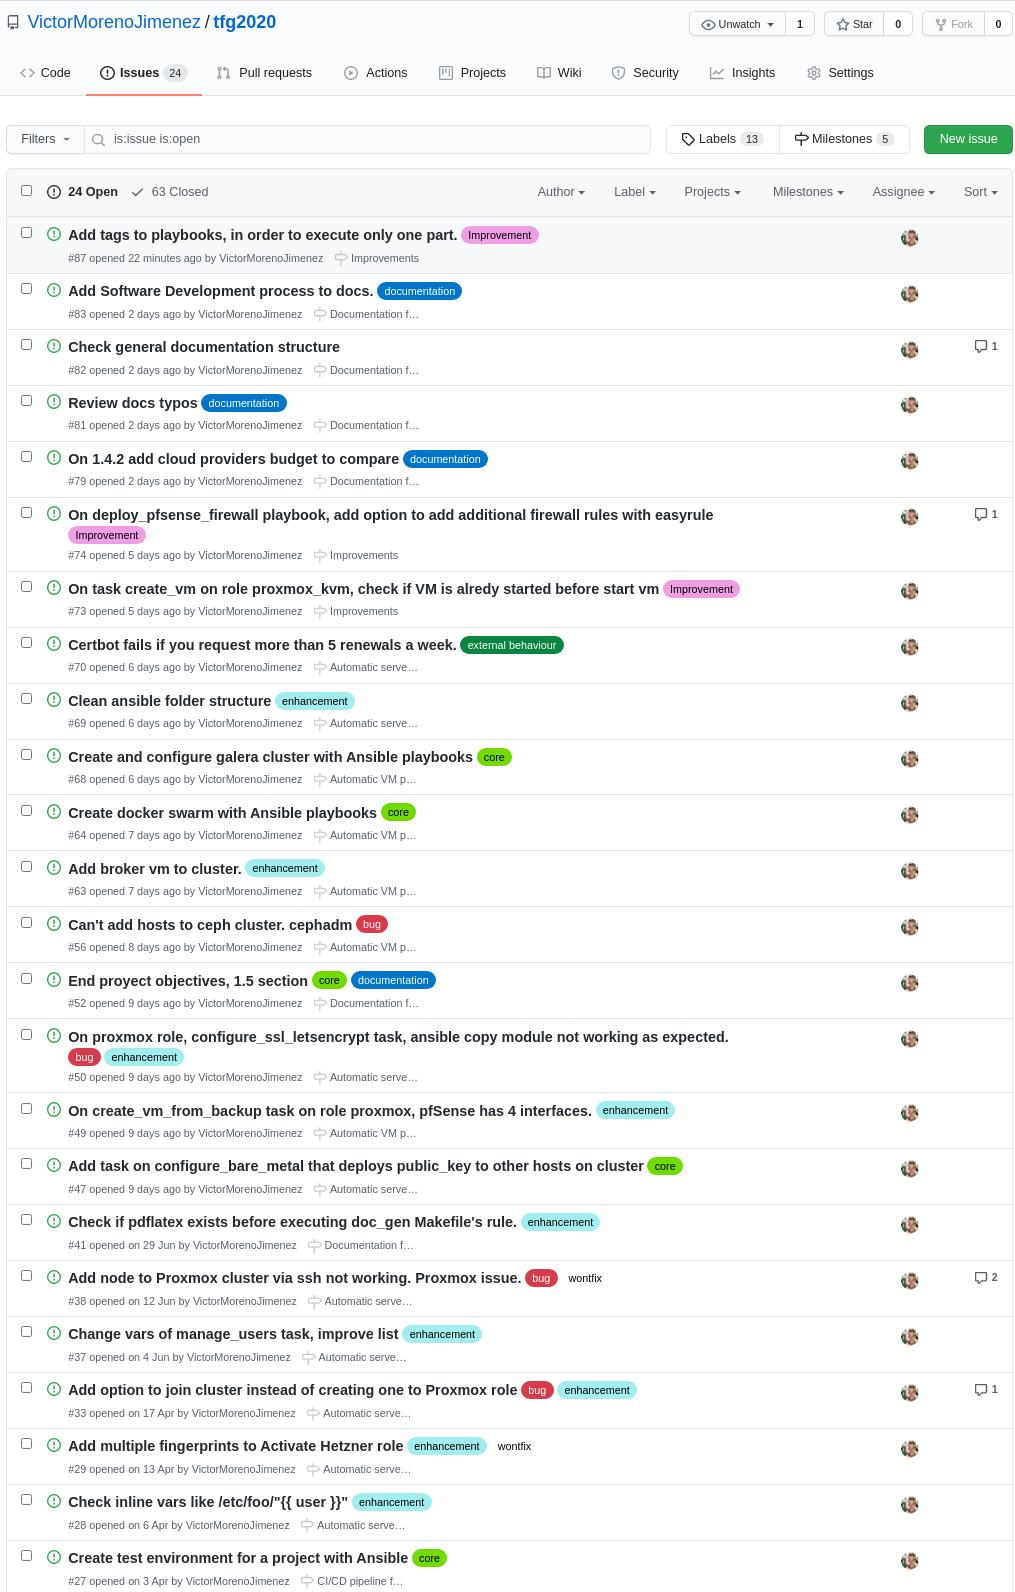
\includegraphics[scale=0.5]{imagenes/Analisis/githubissues.jpg}
		\caption[GitHub panel]{GitHub panel}
		\label{github_issues}
	\end{figure}
\end{text}
\clearpage

\section{Milestones, subjetivos, requisitos funcionales, restricciones e issues}
	\begin{text}
		En el capítulo 1, introducción se definen y detallan los objetivos que este proyecto pretende alcanzar. Sin embargo, estos objetivos presentan un alto grado de abstracción y es difícil trasladarlos a tareas concretas que se traducirán en issues del proyecto. En esta sección vamos a traducir los objetivos principales del proyecto en Milestones, desgranar los objetivos en subobjetivos y traducir cada subobjetivo a un requisito funcional que se convertirá en un issue en el proyecto.
	\end{text}

	\subsection{Milestones}
		\begin{text}
			Los Milestones son estados deseados del proyecto que queremos avanzar para completarlo. Cada Milestone termina un MVP (Minimum Viable Product) y cubre las necesidades de algún objetivo. A continuación se definen los Milestones y se agrupan por objetivos.
			
			\begin{itemize}
				\item \textbf{Milestone 0: Preparar entorno de desarrollo}. Antes de comenzar el proyecto, se debe configurar el equipo que se va a utilizar para trabajar, instalando y configurando el software necesario. 
				\item \textbf{Milestone 1:} Servicio de virtualización desplegado. 
				\item \textbf{Milestone 2:} Cluster seguro.
				\item \textbf{Milestone 3:} Control de versiones en cluster.
				\item \textbf{Milestone 4:} Cluster monitorizado.
				\item \textbf{Milestone 5:} Cluster preparado para desplegar aplicaciones.
				\item \textbf{Milestone 6:} Despliegue automático de aplicaciones.
			\end{itemize}
			A continuación se relaciona cada objetivo definido en la sección \nameref{objetivos_primarios} con su Milestone.
			
		
		\begin{table}[!hbt]
			\begin{tabular}{llllll}
				& Objetivo1         & Objetivo2         & Objetivo3         & Objetivo4         & Objetivo5         \\
				Milestone1 & \textbf{X} & \textbf{X} & \textbf{}  &            &            \\
				Mliestone2 & \textbf{X} & \textbf{X} &            &            &            \\
				Milestone3 &            &            & \textbf{X} & \textbf{X} &            \\
				Milestone4 &            &            & \textbf{X} & \textbf{X} &            \\
				Milestone5 &            &            & X          & \textbf{X} &            \\
				Milestone6 &            &            &            &            & \textbf{X}
			\end{tabular}
		\end{table}
	
		Los Milestones 1,2 están relacionados con la creación y replicación de la infraestructura base, mientras que los Milestones 3,4 y 5 con los servicios desplegados en la infraestructura. Milestone 6 asegura que existen cauces de integración continua y despliegue automático de aplicaciones.
			
		\end{text}

	\subsection{Subobjetivos}
		\begin{text}
			Vamos a analizar cada uno de los objetivos principales con el fin de desgranarlos en subobjetivos que se traduzcan en tareas realizables. 
			\begin{itemize}
				\item \textbf{Objetivo 1}. Asegurar unos tiempos bajos en la creación de infraestructura para proveer servicios.
				\begin{itemize}
					\item \textbf{Subobjetivo 1.1}. Automatización despliegue infraestructura sobre bare metal (tanto este subobjetivo como sus tareas se deben realizar de forma automática con alguna herramienta de automatización).
					\begin{itemize}
						\item Instalar ISO sobre bare metal.
						\item Configuración sistema.
						\item Instalar servicio de virtualización.
						\item Configurar servicio virtualización.
						\item Crear cluster usando el servicio de virtualización.
						\item Agregar los nodos al cluster.
						\item Configurar sistemas de almacenamiento en cluster.
					\end{itemize}
				\end{itemize}
				\item \textbf{Objetivo 2}. Replicar la infraestructura asegurando bajos tiempos de creación. El objetivo 1 cubre las necesidades del objetivo 2. Al crear la infraestructura con herramientas de automatización y estando la infraestructura codificada en ficheros de configuración bajo control de versiones, aseguramos poder replicar la infraestructura en cualquier momento. Al automatizarlo aseguramos mejores tiempos que de forma manual.
				
				\item \textbf{Objetivo 3}. Crear servicios necesarios para una empresa de aplicaciones web asegurando bajos tiempos de creación.
				\begin{itemize}
					\item \textbf{Subobjetivo 3.1}. Automatización despliegue servicios en infraestructura (tanto este subobjetivo como sus tareas se deben realizar de forma automática con alguna herramienta de automatización).
					\begin{itemize}
						\item Desplegar firewall redundante.
						\item Desplegar servicio de control de versiones.
						\item Desplegar servicio de almacenamiento estático.
						\item Desplegar servicio gestión aplicaciones.
						\item Desplegar servicio orquestación contenedores.
						\item Desplegar servicio de servidor web.
						\item Desplegar servicio de base de datos.
						\item Desplegar servicio de monitorización.
						\item Desplegar servicio gestor de colas.
					\end{itemize}
				\end{itemize}
				\item \textbf{Objetivo 4}. Replicar cualquier servicio alojado en la infraestructura de una empresa en la infraestructura de forma rápida. Al igual que pasa con los objetivos 1 y 2, los objetivos 3 y 4 están relacionados y si se cumple 3 se cumple 4. Si conseguimos automatizar la creación de los servicios con ficheros de configuración bajo control de versiones, aseguramos el poder replicarlos en cualquier momento.
				\item \textbf{Objetivo 5}. Crear cauces rápidos y seguros para la creación de nuevo software.
				\begin{itemize}
					\item \textbf{Subobjetivo 5.1}. Automatización despliegue aplicaciones con integración continua.
					\begin{itemize}
						\item Instalación y configuración servicio CI + CD.
						\item Adaptación proyecto a CI/CD (tests).
						\item Creación de los cauces en servicio elegido.
					\end{itemize}
				\end{itemize}
			\end{itemize}
		\end{text}
	
	\subsection{Requisitos funcionales}
	\begin{itemize}
		\item \textbf{RF 0.} El sistema permitirá la automatizar la configuración del equipo del sistema que va a utilizar el proyecto para la configuración de sistemas remotos.
		\item \textbf{RF 1.} El sistema permitirá la automatizar la creación de la infraestructura.
		\begin{itemize}
			\item \textbf{RF 1.1}. El sistema permitirá automatizar ĺa instalación de una ISO elegida sobre el servidor.
			\item \textbf{RF 1.2}. El sistema permitirá automatizar ĺa instalación de una ISO elegida sobre el servidor.
			\item \textbf{RF 1.3}. El sistema permitirá la instalación de un servicio de virtualización. 
			\item \textbf{RF 1.4}. El sistema permitirá la configuración de un servicio de virtualización.
			\item \textbf{RF 1.5}. El sistema permitirá la creación de un cluster sobre el servicio de virtualización.
			\item \textbf{RF 1.6}. El sistema permitirá añadir nuevos nodos al cluster.
			\item \textbf{RF 1.7}. El sistema permitirá configurar los sistemas de almacenamiento utilizados por el cluster.
		\end{itemize}
		\item \textbf{RF 2.} El sistema permitirá la replicación de la infraestructura.
		\item \textbf{RF 3.} El sistema permitirá la creación de los servicios necesarios para una empresa de desarrollo web.
		\begin{itemize}
			\item \textbf{RF 3.1}. El sistema permitirá la creación de un servicio de firewall en el cluster. (RNF 4)
			\item \textbf{RF 3.2}. El sistema permitirá la creación de un servicio de control de versiones en el cluster.
			\item \textbf{RF 3.3}. El sistema permitirá la creación de un servicio de almacenamiento estático en el cluster.
			\item \textbf{RF 3.4}. El sistema permitirá la creación de un servicio de gestión de aplicaciones Wordpress en el cluster.
			\item \textbf{RF 3.5}. El sistema permitirá la creación de un servicio de orquestación de contenedores en el cluster. (RNF 4)
			\item \textbf{RF 3.6}. El sistema permitirá la creación de un servicio de servidor web en el cluster.
			\item \textbf{RF 3.7}. El sistema permitirá la creación de un servicio de monitorización en el cluster.
			\item \textbf{RF 3.8}. El sistema permitirá la creación de un servicio de base de datos en el cluster. (RNF 3)
			\item \textbf{RF 3.9}. El sistema permitirá la creación de un servicio de gestión de colas.
		\end{itemize}
	
	\item \textbf{RF 4}. El sistema permitirá la recreación de infraestructura en un tiempo bajo.
	
	\item \textbf{RF 5}. El sistema permitirá el despliegue automatizados en un cluster seguro.
	\end{itemize}

	\subsection{Requisitos funcionales}
	\begin{itemize}
		\item \textbf{RNF 1}. El sistema debe garantizar la automatización de los procesos de creación de infraestructura.
		\item \textbf{RNF 2}. El sistema debe garantizar la automatización de los procesos de creación de servicios en la infraestructura.
		\item \textbf{RNF 3}. El sistema debe garantizar la alta disponibilidad de el servicio de base de datos.
		\item \textbf{RNF 4}. El sistema debe garantizar la alta disponibilidad de las aplicaciones.
	\end{itemize}

	\subsection{Restricciones}
	\begin{text}
		Este proyecto se ha desarrollado para una empresa en concreto y se realiza sobre una base. Esto conlleva restricciones a la hora de elegir las tecnologías a utilizar para satisfacer los objetivos. A continuación se listan las restricciones tecnológicas que presenta este proyecto.
		
		\begin{itemize}
			\item \textbf{Restricción 1.} El uso de las siguientes tecnologías será necesario para la correcta adaptación del proyecto a la empresa:
			\begin{itemize}
				\item Bases de datos: MySQL
				\item Almacenamiento estático: Ceph cluster
				\item Servicio virtualización: Proxmox
				\item Servido web: Nginx
				\item Contenedores: Docker
				\item Firewall: pfSense
				\item Control de versiones: GitLab
				\item Proyectos: Django + Angular \& Wordpress
			\end{itemize}
		\end{itemize}
	\end{text}

	\subsection{Tecnologías elegidas}
	\begin{text}
		Las tecnologías que se van a utilizar en la infraestructura y los servicios de el proyecto están bien definidas y son una restricción impuesta por la empresa, sin embargo para lograr el objetivo de este proyecto, hace falta elegir la herramienta de automatización que se va a elegir. A continuación se va a hacer un análisis de las principales herramientas disponibles, pros y contras de cada una y el por qué se ha elegido la tecnología utilizada.
	\end{text}
	\subsubsection{Puppet}
	\begin{text}
		Puppet es una herramienta de software libre de gestión de configuración de software. Es comúnmente utilizado por los administradores de sistemas para configurar múltiples servidores y para automatizar las tareas de mantenimiento. Puppet se adapta perfectamente a las necesidades de este proyecto. Sin embargo, la complejidad del lenguaje ruby junto con la necesidad de crear una infraestructura maestro - esclavo con los distintos nodos hace que se haya desechado esta opción.
	\end{text}
\clearpage
	\subsubsection{Chef}
	\begin{text}
		Chef es una herramienta open source con objetivos similares a Puppet. Basado en ruby y orientado a desarrolladores con experienca en ruby. La curva de aprendizaje es menor que la de Puppet. Sin embargo, también hay que crear una infraestructura específica para usar Chef con un nodo que actuaria de servidor y los nodos esclavos que serían los servidores a configurar.
	\end{text}
	\subsubsection{Ansible}
	\begin{text}
		Por último la elegida, Ansible. Ansible está basado en python y también es software libre. La gran ventaja de Ansible frente a Chef o Puppet es que no necesitamos generar ninguna estructura específica dentro del sistema para ejecutar tareas de Ansible. Simplemente instalar Ansible y los módulos necesarios según nuestras necesidades. También aprender Ansible es bastante asequible ya que los playbooks o ficheros de configuración Ansible son ficheros .yml. Los playbooks se ejecutan en orden secuencial lo que facilita mucho su comprensión. Es por todo esto que hemos elegido Ansible como herramienta de automatización para cumplir con los objetivos de este proyecto.
	\end{text}
	
	\subsection{Issues}
	\begin{text}
		A continuación se van a redactar los issues necesarios para cumplir con los requisitos funcionales. Se van a agrupar estos issues en Milestones.
		
		\begin{itemize}
			\item \textbf{Milestone 0:} Entorno de desarrollo. 
				\begin{itemize}
					\item \textbf{Issue 0.1}. Crear playbooks de Ansible para configurar el equipo de desarrollo.
					\item \textbf{Issue 0.2} Crear playbooks de Ansible para crear la estructura de carpetas necesaria para el proyecto.
				\end{itemize}
			\item \textbf{Milestone 1:} Servicio de virtualización desplegado. 
				\begin{itemize}
					\item \textbf{Issue 1.1}. Automatizar instalación ISO en servidores Hetzner con rescue mode activado.
					\item \textbf{Issue 1.2}. Automatizar configuración LVM sobre ISO instalada.
					\item \textbf{Issue 1.3}. Automatizar instalación paquetes en los nodos.
					\item \textbf{Issue 1.4}. Automatizar gestión de usuarios/grupos del sistema en los nodos.
					\item \textbf{Issue 1.5}. Automatizar la instalación de servicio de virtualización Proxmox en los nodos.
					\item \textbf{Issue 1.6}. Automatizar gestión de usuarios/grupos Proxmox en los nodos.
					\item \textbf{Issue 1.7}. Automatizar gestión de almacenamiento Proxmox en los nodos.
					\item \textbf{Issue 1.8}. Automatizar creación e instalación certificado SSL en los nodos.
					\item \textbf{Issue 1.9}. Automatizar la creación del cluster Proxmox.
					\item \textbf{Issue 1.10}. Automatizar la adición de nuevos nodos al cluster.
				\end{itemize}
			\item \textbf{Milestone 2:} Cluster seguro.
				\begin{itemize}
					\item \textbf{Issue 2.1}. Automatizar creación de máquina virtual pfSense en servicio de virtualización Proxmox.
					\item \textbf{Issue 2.2}. Modificar puerto SSH para poder ejecutar playbook sobre pfSense.
					\item \textbf{Issue 2.3}. Automatizar la configuración del firewall pfSense.
					\item \textbf{Issue 2.4}. Permitir la modificación de la configuración pfSense a través de un playbook de Ansible.
				\end{itemize}
			\item \textbf{Milestone 3:} Control de versiones en cluster.
				\begin{itemize}
					\item \textbf{Issue 3.1}. Automatizar la creación de máquina virtual en cluster donde instalar GitLab.
					\item \textbf{Issue 3.2}. Instalar GitLab en máquina virtual Proxmox.
					\item \textbf{Issue 3.3}. Configurar pfSense DHCP, añadir nueva IP.
					\item \textbf{Issue 3.4}. Automatizar configuración GitLab mediante ficheros de configuración.
				\end{itemize}
			\item \textbf{Milestone 4:} Cluster monitorizado.
				\begin{itemize}
					\item \textbf{Issue 4.1}. Automatizar la creación de máquina virtual en cluster donde instalar Icinga2.
					\item \textbf{Issue 4.2}. Instalar Icinga2 en máquina virtual Proxmox.
					\item \textbf{Issue 4.3}. Configurar pfSense DHCP, añadir nueva IP.
					\item \textbf{Issue 4.4}. Instalar Icinga2 Director sobre Icinga 2.
				\end{itemize}
			\item \textbf{Milestone 5:} Cluster preparado para desplegar aplicaciones.
				\begin{itemize}
					\item \textbf{Issue 5.1}. Instalar y configurar Ceph cluster.
					\item \textbf{Issue 5.2}. Instalar y configurar Galera cluster.
					\item \textbf{Issue 5.3}. Instalar y configurar Virtualmin.
					\item \textbf{Issue 5.4}. Instalar y configurar Kubernetes cluster.
					\item \textbf{Issue 5.5}. Instalar y configurar RabbitMQ.
					\item \textbf{Issue 5.6}. Instalar y configurar Nginx.
				\end{itemize}
			\item \textbf{Milestone 6:} Despliegue automático de aplicaciones.
				\begin{itemize}
					\item \textbf{Issue 6.2}. Dockerizar proyecto Djagno + Angular.
					\item \textbf{Issue 6.2}. Creación test unitarios.
					\item \textbf{Issue 6.1}. Instalación y configuración de GiLab CI+CD.
					\item \textbf{Issue 6.3}. Adaptar proyecto a CI/CD.
				\end{itemize}
		\end{itemize}
	\end{text}



%\section{Tipos de usuario}
%	\begin{text}
%		Adoptando la filosofía DevOps, tanto desarrolladores como sysadmin debería adoptar el mismo rol. Sin embargo, en una empresa en la cual crean y configuran sus propios servidores sin contratar servicios externos (como Azure DevOps, AWS...) se crea la necesidad de crear y configurar la infraestructura que va a alojar toda la infraestructura necesaria para el desarrollo cada aplicación. Es por esto que se distinguen entre dos tipos de usuarios: \textbf{Desarrolladores} y \textbf{Sistemas + Desarrolladores}.  
		
%		\begin{itemize}
%			\item \textbf{Desarrolladores}. Este tipo usuario tiene las siguientes necesidades:
%				\item Poder construir una infraestructura para el desarrollo de aplicaciones bajo demanda. [RF 1]
%				\item Poder integrar cambios a las aplicaciones. [RF 2]
%				\item Poder tener feedback de el estado de la aplicación tras el despliegue. [RF 3]
%				\item Conocer la configuración del servidor donde se aloja la aplicación web. [RF 4]
%			\item \textbf{Desarrolladores + Sistemas}
%				\item Poder construir una infraestructura para el desarrollo de aplicaciones bajo d%emanda. [RF 1]
%				\item Poder integrar cambios a las aplicaciones. [RF 2]
%%				\item Poder tener feedback de el estado de la aplicación tras el despliegue. [RF 3]
%				\item Conocer la configuración del servidor donde se aloja la aplicación web. [RF 4]
%				\item Poder desplegar la infraestructura completa que aloja la infraestructura para las aplicaciones. [RF 5]
%				\item Poder conocer la configuración de la infraestructura. [RF 6]
%		\end{itemize}
	
%		Estos historias de usuario representan la funcionalidad final del proyecto, con un nivel de abstracción muy alto. En la siguiente sección, se desgranarán estas historias para definir de forma precisa los requisitos funcionales. \cite{ReqF:online} 
%	\end{text}

%\section{Especificación de requisitos}
%	\label{erf}
%	\begin{text}
%		A continuación se detallan los requisitos funcionales de este proyecto. 
%		\begin{itemize}
%			\item Construir y desplegar infraestructura para el desarrollo de aplicaciones bajo demanda. [RF 1]
%			\item Poder integrar cambios en las aplicaciones de forma autónoma [RF 2]
%			\item Conocer el estado de la aplicación una vez hecho el despliegue [RF 3]
%%			\item Conocer la configuración del servidor donde se aloja la aplicación web. [RF 4]
%			\item Poder desplegar la infraestructura completa que aloja la infraestructura para las aplicaciones a través de ficheros de configuración. [RF 5]
%			\item Conocer en todo momento la configuración del servidor [RF 6]
%			\item Poder desplegar la infraestructura rápidamente ante un error catastrófico [RF 7]
%			\item Realizar tareas de mantenimiento en los servidores con tareas automatizadas [RF 8]
%			\item Crear máquinas virtuales bajo demanda con tareas automatizadas y ficheros de configuración [RF 9]
%			\item Modificar la configuración de los firewall con tareas automatizadas [RF 10]
%		\end{itemize}
%	\end{text}

%section{Diagramas}
%	\subsection{Diagramas casos de uso}
%		\begin{text}
%			A continuación se muestran los principales diagramas según los requisitos funcionales descritos en la sección \nameref{erf}.
%		\end{text}
	
%		\begin{figure}[!hbt]
%			\centering
%			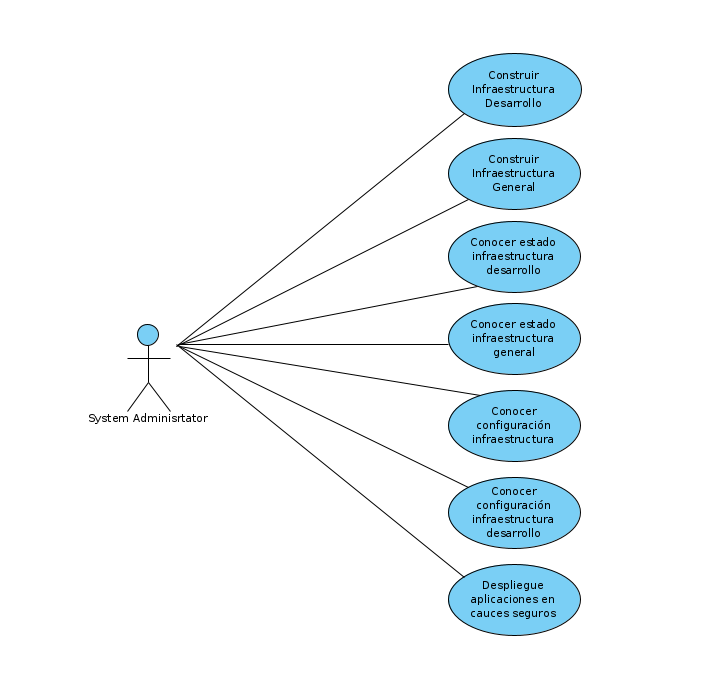
\includegraphics[scale=0.4]{imagenes/Analisis/casos_uso_administrador.png}
%			\caption[Casos de uso Administrador]{Casos de uso \cite{casosuso:online}} 
%			\label{Casos de uso Administrador}
%		\end{figure}
	
%		\begin{figure}[!hbt]
%			\centering
%			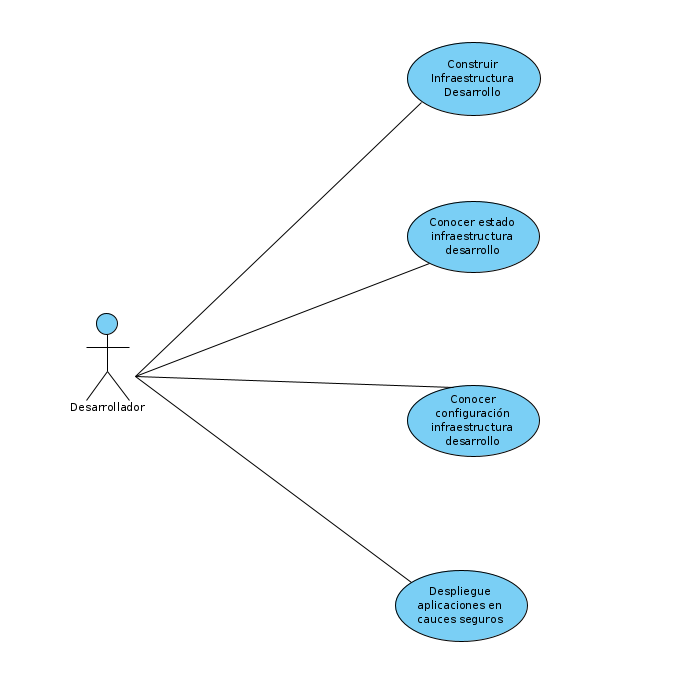
\includegraphics[scale=0.4]{imagenes/Analisis/casos_uso_desarrollador.png}
%			\caption[Casos de uso Desarrollador]{Casos de uso \cite{casosuso:online}} 
%			\label{Casos de uso Desarrollador}
%		\end{figure}
	
%	\subsection{Diagramas de secuencia}
%		\begin{figure}[!hbt]
%			\centering
%			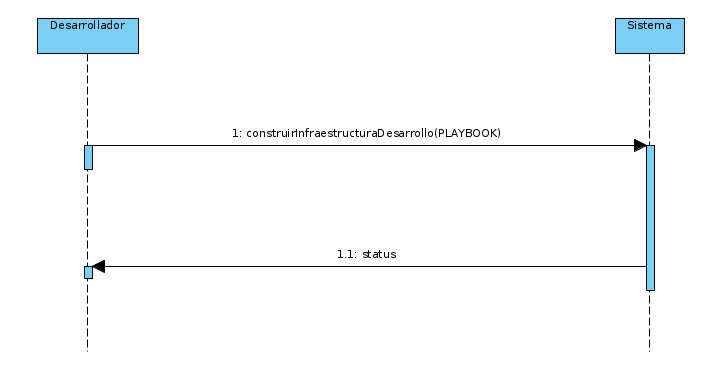
\includegraphics[scale=0.4]{imagenes/Analisis/diagrama_secuencia_desarrollador_1.png}
%			\caption[Diagrama secuencia Desarrollador 1]{Diagrama secuencia Desarrollador 1 %cite{diagramasecuencia:online}} 
%			\label{Diagrama secuencia_desarrollador_1}
%		\end{figure}
%		\clearpage
	
%		\begin{figure}[!hbt]
%			\centering
%			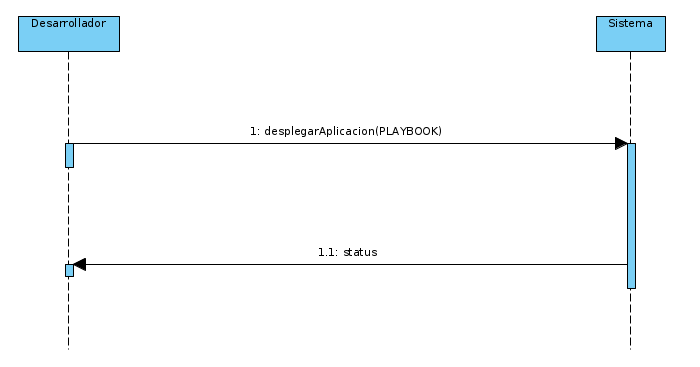
\includegraphics[scale=0.4]{imagenes/Analisis/diagrama_secuencia_desarrollador_4.png}
%			\caption[Diagrama secuencia Desarrollador 2]{Diagrama secuencia Desarrollador 2 \cite{diagramasecuencia:online}} 
%			\label{Diagrama secuencia_desarrollador_2}
%		\end{figure}

%		\begin{figure}[!hbt]
%			\centering
%			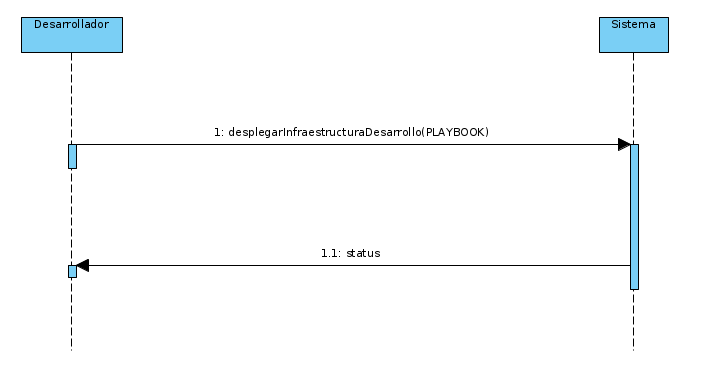
\includegraphics[scale=0.4]{imagenes/Analisis/diagrama_secuencia_desarrollador_3.png}
%			\caption[Diagrama secuencia Desarrollador 3]{Diagrama secuencia Desarrollador 3 \cite{diagramasecuencia:online}} 
%			\label{Diagrama secuencia_desarrollador_3}
%		\end{figure}
	
%		\begin{figure}[!hbt]
%			\centering
%			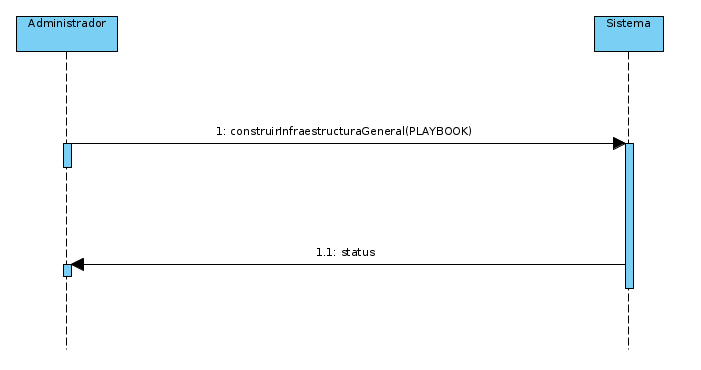
\includegraphics[scale=0.4]{imagenes/Analisis/diagrama_secuencia_administrador_1.png}
%			\caption[Diagrama secuencia Administrador 1]{Diagrama secuencia Administrador 1 \cite{diagramasecuencia:online}}
%			\label{Diagrama secuencia_administrador_1}
%		\end{figure}
%		\clearpage
		
%		\begin{figure}[!hbt]
%			\centering
%			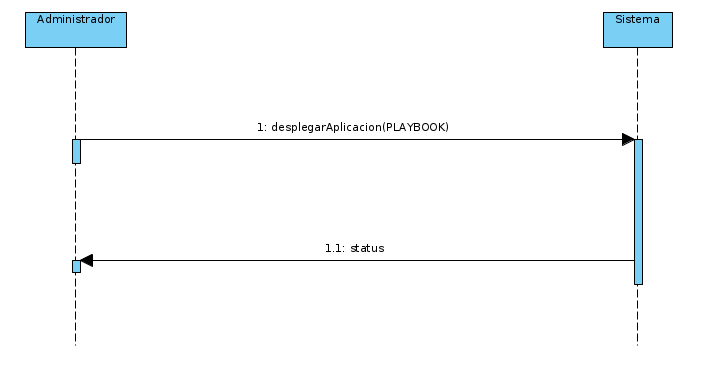
\includegraphics[scale=0.4]{imagenes/Analisis/diagrama_secuencia_administrador_2.png}
%			\caption[Diagrama secuencia Administrador 2]{Diagrama secuencia Administrador 2 \cite{diagramasecuencia:online}}
%			\label{Diagrama secuencia_administrador_2}
%		\end{figure}
	
%		\begin{figure}[!hbt]
%			\centering
%			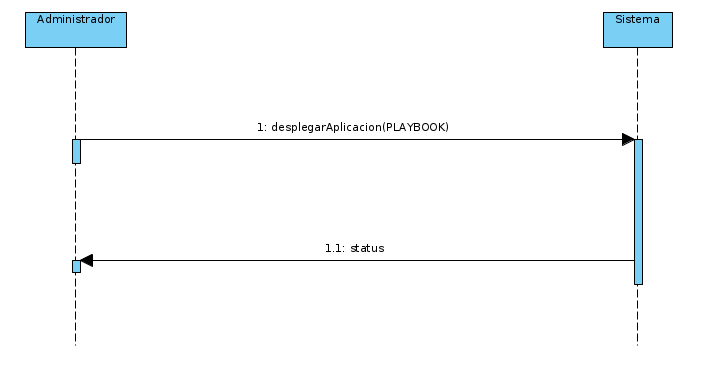
\includegraphics[scale=0.4]{imagenes/Analisis/diagrama_secuencia_administrador_2.png}
%			\caption[Diagrama secuencia Administrador 3]{Diagrama secuencia Administrador 3 \cite{diagramasecuencia:online}}
%			\label{Diagrama secuencia_administrador_3}
%		\end{figure}
		
%\clearpage
\section{Casos de uso}

	\begin{usecase}{Configurar entorno proyecto << CU.0 >>}
		\addrow{Descripción}{Configura el equipo donde se van a lanzar las tareas del proyecto.}
		
		\addrow{Actores}{Administrador/Desarrollador}
		
		\addrow{Precondición}{El usuario dispone de un equipo con una ISO instalada de la familia Debian.}
		
		\addrow{Postcondición}{El equipo del usuario queda preparado para la ejecución de tareas del proyecto.}
		
		\addmulrow{Secuencia principal (P)}{
			\item El usuario clona el proyecto
			\item El usuario configura las va- \\
			riables necesarias para ejecutar el \\ 
			playbook
			\item El usuario ejecuta el playbook \\ \textbf{configure\_development\_\\environment} 
			\item El sistema ejecuta las tareas en el \\
			equipo local
			\item El sistema informa al usuario \\
			del resultado de la ejecución}
		\hline
	\end{usecase}
	\clearpage
	\begin{usecase}{Crear infraestructura << CU.1 >>}
		\addrow{Descripción}{Permite crear la infraestructura sobre los nodos.}
		
		\addrow{Actores}{Administrador}
		
		\addrow{Precondición}{El usuario administrador ha clonado el proyecto y ha configurado correctamente los ficheros hosts.yml, asignado valor a las variables de los roles hetzner y proxmox\_nodes y ejecutado caso de uso 0}
		
		\addrow{Postcondición}{Los nodos están configurados con la ISO elegida instalada y el servicio de virtualización Proxmox desplegado. Creado y configurado cluster Proxmox.}
		
		\addmulrow{Secuencia principal (P)}{
			\item El administrador clona el proyecto
			\item El administrador configura las va- \\
				riables necesarias para ejecutar el \\ 
				playbook
			\item El administrador ejecuta el play- \\
			book \textbf{configure\_proxmox\_nodes} 
			\item El sistema ejecuta las tareas en los \\
				nodos 
			\item El sistema informa al administrador \\
				  del resultado de la ejecución}
			  \hline
	\end{usecase}
	\clearpage
	\begin{usecase}{Replicar infraestructura << CU.2 >>}
		\addrow{Descripción}{Permite replicar la infraestructura sobre los nodos.}
		
		\addrow{Actores}{Administrador}
		
		\addrow{Precondición}{El usuario administrador ha clonado el proyecto y ha configurado correctamente el fichero hosts.yml con los nuevos nodos donde replicar la infraestructura, asignado valor a las variables de los roles hetzner y proxmox\_nodes y ejecutado caso de uso 0}
		
		\addrow{Postcondición}{La infraestructura desplegada en << CU.1 >> queda replicada en los nodos elegidos.}
		
		\addmulrow{Secuencia principal (P)}{
			\item El administrador clona el proyecto
			\item El administrador configura las va- \\
			riables necesarias para ejecutar el \\ 
			playbook
			\item El administrador ejecuta el play- \\
			book \textbf{configure\_proxmox\_nodes} 
			\item El sistema ejecuta las tareas en los \\
			nodos 
			\item El sistema informa al administrador \\
			del resultado de la ejecución}
 
		\hline
	\end{usecase}
	\clearpage
	
	\begin{usecase}{Crear servicio firewall << CU.3 >>}
		\addrow{Descripción}{Permite crear un servicio de firewall en el cluster.}
		
		\addrow{Actores}{Administrador}
		
		\addrow{Precondición}{El usuario ha ejecutado correctamente << CU.0 >> y  << CU.1 >> o << CU.2 >>}
		
		\addrow{Postcondición}{Se ha creado el servicio de firewall pfSense en el cluster.}
		
		\addmulrow{Secuencia principal (P)}{
			\item El administrador ejecuta \\ correctamente << CU.0 >>
			\item El administrador ejecuta \\ correctamente  << CU.1 >> \\
			o << CU.2 >>.
			\item El administrador configura \\ variables 
			de role \textbf{pfsense} 
			\item El administrador ejecuta playbook \\  
				\textbf{deploy\_pfsense\_firewall}
			\item El sistema ejecuta las tareas en los \\
			nodos. 
			\item El sistema informa al administrador \\
			del resultado de la ejecución}
		\hline
	\end{usecase}
\clearpage
\begin{usecase}{Crear servicio almacenamiento estático << CU.4 >>}
	\addrow{Descripción}{Permite crear un servicio de almacenamiento estático en el cluster.}
	
	\addrow{Actores}{Administrador}
	
	\addrow{Precondición}{El usuario ha ejecutado correctamente << CU.0 >> y  << CU.1 >> o << CU.2 >> y << CU.3 >>}
	
	\addrow{Postcondición}{Se ha creado el servicio de almacenamiento estático \textbf{Ceph cluster} en el cluster.}
	
	\addmulrow{Secuencia principal (P)}{
		\item El administrador ejecuta \\ correctamente << CU.0 >>
		\item El administrador ejecuta \\ correctamente  << CU.1 >> \\
		o << CU.2 >> y << CU.3 >>.
		\item El administrador configura \\ variables 
		de role \textbf{pfsense} 
		\item El administrador ejecuta playbook \\  
		\textbf{deploy\_pfsense\_firewall}
		\item El sistema ejecuta las tareas en los \\
		nodos. 
		\item El sistema informa al administrador \\
		del resultado de la ejecución}
	\hline
\end{usecase}

\begin{usecase}{Crear servicio de gestión de aplicaciones Wordpress << CU.5 >>}
	\addrow{Descripción}{Permite crear un servicio de gestión de aplicaciones Wordpress en el cluster.}
	
	\addrow{Actores}{Administrador}
	
	\addrow{Precondición}{El usuario ha ejecutado correctamente << CU.0 >> y  << CU.1 >> o << CU.2 >> y << CU.3 >>}
	
	\addrow{Postcondición}{Se ha creado el servicio de gestión de aplicaciones Wordpress en el cluster.}
	
	\addmulrow{Secuencia principal (P)}{
		\item El administrador ejecuta \\ correctamente << CU.0 >>
		\item El administrador ejecuta \\ correctamente  << CU.1 >> \\
		o << CU.2 >> y << CU.3 >>.
		\item El administrador configura \\ variables 
		de role \textbf{virtualmin} 
		\item El administrador ejecuta playbook \\  
		\textbf{create\_virtualmin}
		\item El sistema ejecuta las tareas en los \\
		nodos. 
		\item El sistema informa al administrador \\
		del resultado de la ejecución}
	\hline
\end{usecase}

\clearpage 

\begin{usecase}{Crear servicio de orquestación de contenedores en el cluster << CU.6 >>}
	\addrow{Descripción}{Permite crear un servicio de orquestación de contenedores en el cluster en el cluster.}
	
	\addrow{Actores}{Administrador}
	
	\addrow{Precondición}{El usuario ha ejecutado correctamente << CU.0 >> y  << CU.1 >> o << CU.2 >> y << CU.3 >>}
	
	\addrow{Postcondición}{Se ha creado el servicio de orquestación de contenedores en el cluster.}
	
	\addmulrow{Secuencia principal (P)}{
		\item El administrador ejecuta \\ correctamente << CU.0 >>
		\item El administrador ejecuta \\ correctamente  << CU.1 >> \\
		o << CU.2 >> y << CU.3 >>.
		\item El administrador configura \\ variables 
		de role \textbf{kubernetes} 
		\item El administrador ejecuta playbook \\  
		\textbf{create\_kubernetes\_cluster}
		\item El sistema ejecuta las tareas en los \\
		nodos. 
		\item El sistema informa al administrador \\
		del resultado de la ejecución}
	\hline
\end{usecase}

\clearpage

\begin{usecase}{Crear servicio de monitorización en el cluster << CU.7 >>}
	\addrow{Descripción}{Permite crear un servicio de monitorización en el cluster.}
	
	\addrow{Actores}{Administrador}
	
	\addrow{Precondición}{El usuario ha ejecutado correctamente << CU.0 >> y  << CU.1 >> o << CU.2 >> y << CU.3 >>}
	
	\addrow{Postcondición}{Se ha creado el servicio de monitorización en el cluster.}
	
	\addmulrow{Secuencia principal (P)}{
		\item El administrador ejecuta \\ correctamente << CU.0 >>
		\item El administrador ejecuta \\ correctamente  << CU.1 >> \\
		o << CU.2 >> y << CU.3 >>.
		\item El administrador configura \\ variables 
		de role \textbf{icinga2}.
		\item El administrador ejecuta playbook \\  
		\textbf{create\_icinga2}.
		\item El sistema ejecuta las tareas en los \\
		nodos. 
		\item El sistema informa al administrador \\
		del resultado de la ejecución}
	\hline
\end{usecase}

\clearpage

\begin{usecase}{Crear servicio de bases de datos << CU.8 >>}
	\addrow{Descripción}{Permite crear un servicio bases de datos en el cluster.}
	
	\addrow{Actores}{Administrador}
	
	\addrow{Precondición}{El usuario ha ejecutado correctamente << CU.0 >> y  << CU.1 >> o << CU.2 >> y << CU.3 >>}
	
	\addrow{Postcondición}{Se ha creado el servicio de bases de datos en el cluster.}
	
	\addmulrow{Secuencia principal (P)}{
		\item El administrador ejecuta \\ correctamente << CU.0 >>
		\item El administrador ejecuta \\ correctamente  << CU.1 >> \\
		o << CU.2 >> y << CU.3 >>.
		\item El administrador configura \\ variables 
		de role \textbf{icinga2} 
		\item El administrador ejecuta playbook \\  
		\textbf{create\_galera\_cluster}
		\item El sistema ejecuta las tareas en los \\
		nodos. 
		\item El sistema informa al administrador \\
		del resultado de la ejecución}
	\hline
\end{usecase}

\clearpage 

\begin{usecase}{Crear servicio de gestión de colas << CU.10 >>}
	\addrow{Descripción}{Permite crear un servicio gestión de colas en el cluster.}
	
	\addrow{Actores}{Administrador}
	
	\addrow{Precondición}{El usuario ha ejecutado correctamente << CU.0 >> y  << CU.1 >> o << CU.2 >> y << CU.3 >>}
	
	\addrow{Postcondición}{Se ha creado el servicio de gestión de colas en el cluster.}
	
	\addmulrow{Secuencia principal (P)}{
		\item El administrador ejecuta \\ correctamente << CU.0 >>
		\item El administrador ejecuta \\ correctamente  << CU.1 >> \\
		o << CU.2 >> y << CU.3 >>.
		\item El administrador configura \\ variables 
		de role \textbf{rabbitmq} 
		\item El administrador ejecuta playbook \\  
		\textbf{create\_rabbitmq}
		\item El sistema ejecuta las tareas en los \\
		nodos. 
		\item El sistema informa al administrador \\
		del resultado de la ejecución}
	\hline
\end{usecase}

\clearpage

\begin{usecase}{Recrear infraestructura << CU.11 >>}
	\addrow{Descripción}{Permite replicar infraestructura en nuevos nodos.}
	
	\addrow{Actores}{Administrador}
	
	\addrow{Precondición}{El usuario administrador ha ejecutado correctamente << CU.0 >>, los ficheros hosts.yml con los nodos objetivo y asignado las variables necesarias en os roles \textbf{hetzner}y \textbf{proxmox\_nodes}.}
	
	\addrow{Postcondición}{La infraestructura queda replicada en nuevos nodos.}
	
	\addmulrow{Secuencia principal (P)}{
	\item El administrador ejecuta \\ correctamente << CU.0 >>
	\item El administrador ejecuta \\ correctamente  << CU.1 >> \\
	o << CU.2 >> y << CU.3 >>.
	\item El administrador configura \\ variables 
	de role \textbf{proxmox\_kvm} 
	\item El administrador ejecuta playbook \\  
	\textbf{configure\_proxmox\_nodes}
	\item El sistema ejecuta las tareas en los \\
	nodos. 
	\item El sistema informa al administrador \\
	del resultado de la ejecución}
\hline
\end{usecase}

\clearpage 

\section{Arquitectura del Sistema}
	\subsection{Servidores Físicos}
		\begin{text}
			Al trabajar en una empresa de hosting, he tenido la suerte de contar con 3 servidores bare metal para el desarrollo de este proyecto. Las características técnicas de los servidores se pueden consultar en \nameref{servidores_bare_metal}.
		\end{text}
	\subsection{Infraestructura objetivo}
		\begin{text}
			Este proyecto pretende crear una infraestructura robusta para una pequeña empresa que se dedique al desarrollo del software. Ésta infraestructura debe ser robusta al igual que segura, con lo que ha de proporcionar firewalls redundantes y algún mecanismo para proporcional alta disponibilidad en las aplicaciones web.  A continuación se muestra la infraestructura objetivo.
		\end{text}
	
	\subsection{VSwitch}
	\begin{text}
		El cluster está bajo la red LAN 10.6.0.0/16, de forma que todas las máquinas virtuales están comunicadas. Sin embargo los nodos principales (tfg.intelligenia.com, tfg2.intelligenia.com y tfg3.intelligenia.com) tienen que estar comunicados a través de una red interna para el correcto funcionamiento de Proxmox y los pfSense.
		Es aquí donde entran en juego los switches virtuales de Hetzner. Un VSwitch simula el funcionamiento de un switch convencional, conectando los servidores que se conecten al switch entre sí. De este modo, conseguimos crear una red de conexión entre los nodos principales.
	\end{text}

	\begin{figure}[!hbt]
		\label{InfraestructuraObjetivo}
		\centering
		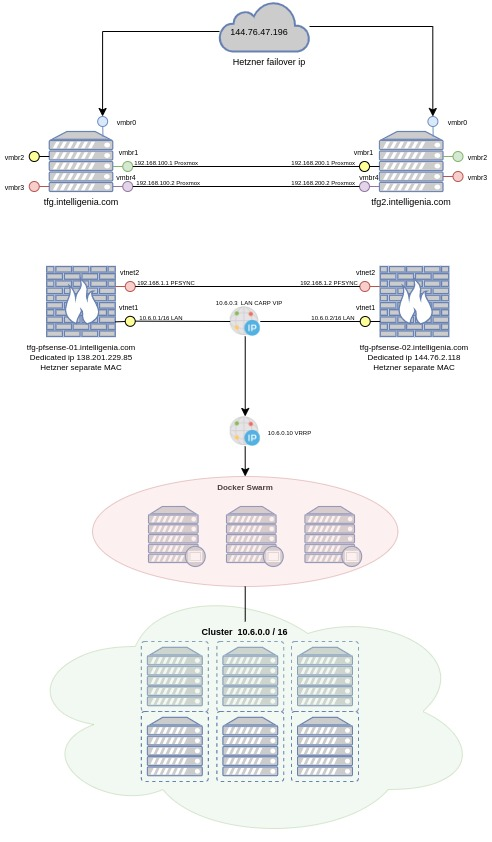
\includegraphics[scale=0.75]{imagenes/Analisis/diagrama.jpg}
		\caption[Infraestructura Objetivo]{Infraestructura Objetivo}
	\end{figure}

	\begin{figure}[!hbt]
		\centering
		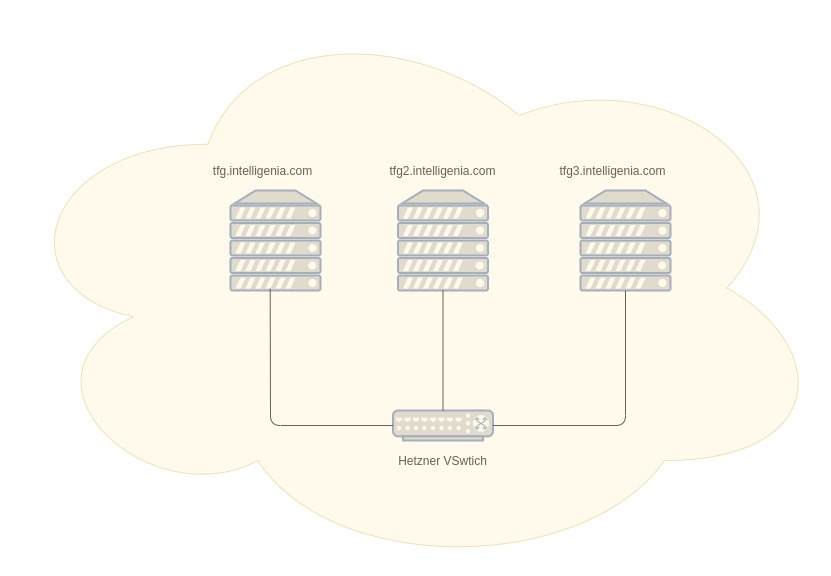
\includegraphics[scale=0.4]{imagenes/Analisis/vswitch.jpg}
		\caption[VSwitch]{VSwitch}
		\label{VSwitch}
	\end{figure}





	
	
	
%
%\chapter {Planificación}

\section{Estimación recursos necesarios}
\begin{text}
	En esta sección se va a crear una estimación de los recursos, tanto humanos como económicos que se van a necesitar para llevar a cabo el proyecto. Cabe destacar que en la estimación temporal se incluye un lapso de tiempo para adaptarse a la tecnología a usar. Ésto no se ha indicado de forma explícita, pero va implícito en estimación temporal de ejecución de cada hito. \\ 
	
\end{text}
\subsection{Estimación temporal}
\begin{text}
	Para dar una estimación del tiempo requerido para el proyecto, vamos a utilizar un diagrama de Gantt, en el que incluiremos los principales hitos del proyecto y una estimación en semanas de la duración del mismo. Una estimación inicial ha sido de 24 semanas en total, a continuación se muestra el diagrama de Gantt.
\end{text}

\newpage
\subsubsection{Diagrama Gantt}
	\begin{figure}[!hbt]
		\centering
		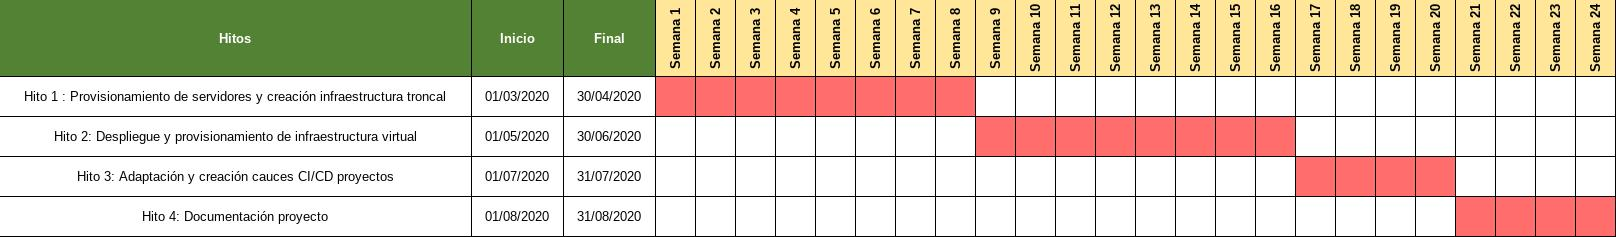
\includegraphics[scale=0.4,angle=-90]{imagenes/Planificacion/gantt.jpg}
		\caption[Diagrama Gantt]{Diagrama Gantt \cite{Gantt:online}} 
		\label{Diagrama Gannt}
	\end{figure}
\clearpage
\section{Presupuesto}
	\begin{text}
		Para realizar este presupuesto, se ha partido del sueldo base de un graduado en Ingeniería Informática. Recalcar que en esta partida, se incluyen horas extra para formación en las tecnologías elegidas.
		Por otra parte se ha incluido en el presupuesto el coste de mantenimiento de la infraestructura.
	\end{text}
	\\
	\begin{table}[ht]
		\centering
		\begin{tabular}[!hbt]{SSSSSSSS} \toprule
			{Concepto} &  {Precio / mes \euro} & {Importe Total \euro} \\ \midrule
			{\textbf{Partida Personal}} \\ \midrule
			{Sueldo DevOps Junior}  & {1.800} & {10.800}  \\
		    \midrule
			{\textbf{Partida Inventariable}} \\ \midrule
			{Coste infraestructura}  & {61,34}  & {368,04}   \\
			\midrule
			{\textbf{Partida Fungible}} \\ \midrule
			{-}  & {-}  & {-}   \\
			\midrule
			{\textbf{Partida servicios técnicos}} \\ \midrule
			{Mantenimiento}  & {Incluido}  & {0} \\
			\midrule	
			{\textbf{Partida viajes y dietas}} \\ \midrule
			{-}  & {-}  & {-} \\
			\midrule	
			{\textbf{Partida de otros}} \\ \midrule
			{Incluido}  & {Incluido}  & {0} \\
			\midrule	
			{\textbf{Total}}  & {1861,34}  & {11.168,04} \\
			\\ \midrule
		 \\ \bottomrule
		\end{tabular}
		\caption[Presupuesto]{Presupuesto \cite{presupuesto:online}} 
		\label{Presupuesto}
	\end{table}

	\begin{text}
		Cabe destacar que en esta partida únicamente se incluyen el coste de un empleado Junior y el coste de la infraestructura necesaria para desarrollar este proyecto. Nótese que en ningún caso, se están añadiendo costes de oficina ni de equipo para desarrollo. En una partida real, habría que incluir estos gastos ya que son imprescindibles para el proceso de desarrollo. En este presupuesto aparece como Otros.
	\end{text}
%
%\input{capitulos/04_Analisis}
%
%\chapter {Diseño}
\section{Arquitectura objetivo}
\subsection{Servidores Físicos}
\begin{text}
	Al trabajar en una empresa de hosting, he tenido la suerte de contar con 3 servidores bare metal para el desarrollo de este proyecto. Las características técnicas de los servidores se pueden consultar en ``\nameref{servidores_bare_metal}''.
\end{text}
\subsection{Infraestructura objetivo}
\label{infraestructura_objetivo}
\begin{text}
	Este proyecto pretende crear una infraestructura para una pequeña empresa que se dedique al desarrollo del software. Esta infraestructura debe ser segura, con lo que ha de proporcionar firewalls redundantes y algún mecanismo para proporcional alta disponibilidad en las aplicaciones web, todo esto está descrito en la sección ``\nameref{objetivos_primarios}''.  A continuación se muestra la infraestructura objetivo. Cabe destacar que las Ips y la información que se muestra en la figura es únicamente de este proyecto con los dominios e IPs contratadas. Sin embargo, la red LAN dentro del cluster sí que se mantendría en otros despliegues del cluster, ya que está no depende de servicios externos. La siguiente figura muestra la estructura general de la infraestructura. Sin embargo, es necesario un nivel de abstracción más bajo para conocer los distintos servicios desplegados en el cluster bajo la red \textbf{10.6.0.0/16}.
	
	\clearpage
	
	\begin{figure}[!hbt]
		\label{InfraestructuraObjetivo}
		\centering
		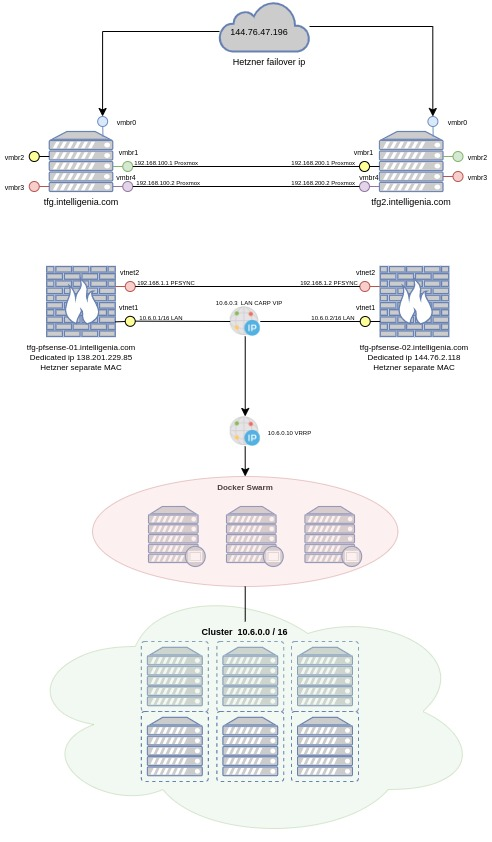
\includegraphics[scale=0.75]{imagenes/Analisis/diagrama.jpg}
		\caption[Infraestructura Objetivo]{Infraestructura Objetivo}
	\end{figure}
\end{text}

\clearpage

\subsection{Diseño Failover}
\begin{text}
	Como se puede apreciar en el diagrama ``\nameref{InfraestructuraObjetivo}'', los dos nodos principales del cluster (los que tienen el firewall) están bajo una \textbf{IP failover}. La IP failover es un tipo especial de IP que puede ir cambiando la IP destino a la que apunta. Esto es imprescindible en un cluster de alta disponibilidad, en nuestro caso si por algún motivo el nodo 1 (tfg.intelligenia.com) al cual apunta la ip failover en un principio sufriera una caída, se activaría un script en el nodo 2 que modificaría el destino de la ip failover y crearía las rutas pertinentes en el nodo 2 para poder recibir todo el tráfico de la IP failover.
	
	Para conseguir esto se ha instalado un pequeño script en los firewall que comprueban constantemente el estado del \textbf{CARP} (Common Address Redundancy Protocol). Esto es lo que permite que a nivel de firewall, haya un maestro y un esclavo. En el momento que el maestro pasa a esclavo o el esclavo pasa a maestro, se ejecuta un script que, utilizando la API de Hetzner modificar el destino de la IP failover.
	
	A continuación se muestra el diagrama que se ha utilizado en los nodos principales para crear el script:
	
	\begin{figure}[!hbt]
		\label{script_failover}
		\centering
		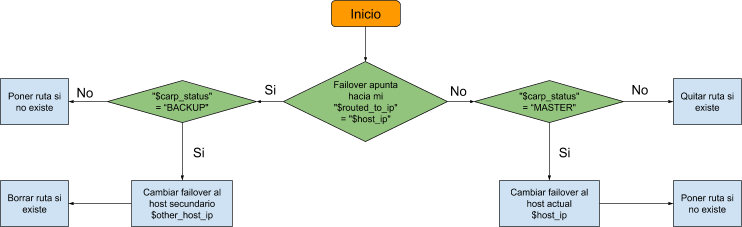
\includegraphics[scale=0.45]{imagenes/Diseno/diagramascript.png}
		\caption[Infraestructura Objetivo]{Infraestructura Objetivo}
	\end{figure}
\end{text}
\clearpage

\subsection{VSwitch}
\begin{text}
	El cluster está bajo la red LAN 10.6.0.0/16, de forma que todas las máquinas virtuales están comunicadas. Sin embargo los nodos principales (tfg.intelligenia.com, tfg2.intelligenia.com y tfg3.intelligenia.com) tienen que estar comunicados a través de una red interna para el correcto funcionamiento de Proxmox y los pfSense.
	Es aquí donde entran en juego los switches virtuales de Hetzner. Un VSwitch simula el funcionamiento de un switch convencional, conectando los servidores que se conecten al switch entre sí. De este modo, conseguimos crear una red de conexión entre los nodos principales.
	
	\begin{figure}[!hbt]
		\centering
		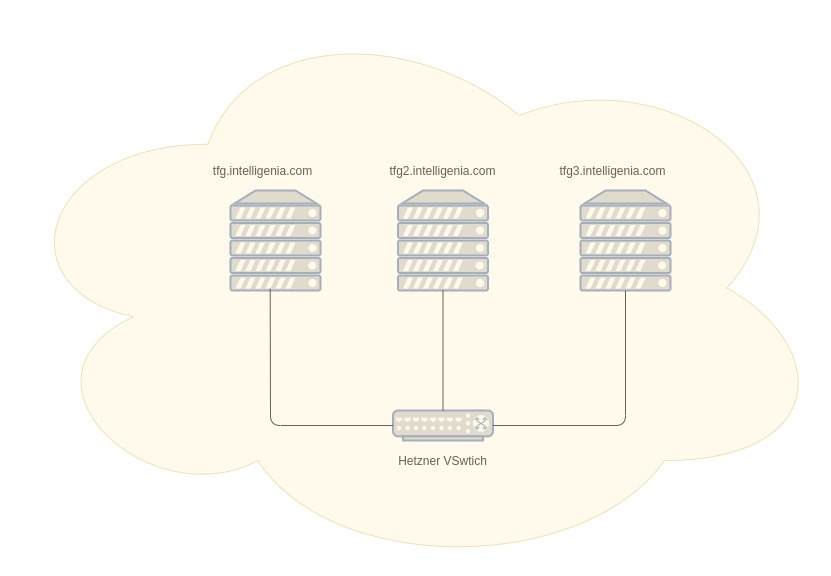
\includegraphics[scale=0.4]{imagenes/Analisis/vswitch.jpg}
		\caption[VSwitch]{VSwitch}
		\label{VSwitch}
	\end{figure}
\end{text}

\begin{text}
	La infraestructura anterior junto con los cauces pertinentes para la integración y despliegues continuos, es lo que pretende este proyecto. A continuación se explica como se ha diseñado la solución que satisface los requisitos funcionales relacionados con lac reación y despliegue de infraestructura con la herramienta de automatización Ansible.
\end{text}
\clearpage

\subsection{Diagrama Cluster}

\begin{text}
	La siguiente figura muestra el cluster con un nivel de abstracción más bajo. Se muestran los distintos servicios que ofrece y la relación entre ellos. Cada servicio desplegado contribuye a la realización de uno o más requisitos funcionales descritos en la sección ``\nameref{requisitosfuncionales}'' cucho propósito es lograr los objetivos definidos en ``\nameref{subobjetivos}''. \\
	El cluster de servicios está interconectado entre sí en la red \textbf{10.6.100.0/24}.
\end{text}
\begin{figure}[!hbt]
	\centering
	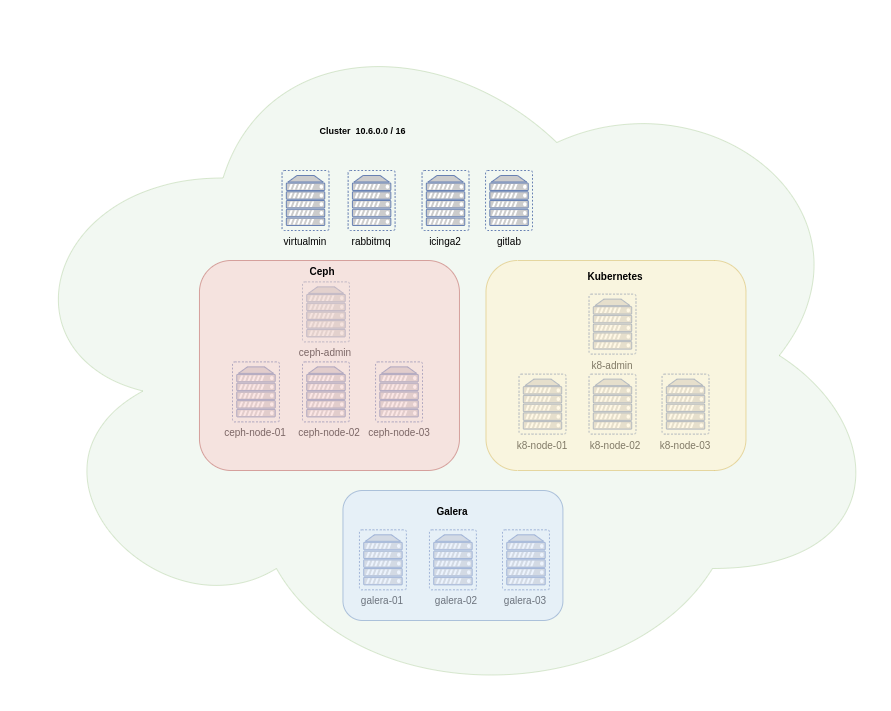
\includegraphics[scale=0.40]{imagenes/Diseno/diagrama_cluster_2.png}
	\caption[Diseño Cluster]{Diseño Cluster} 
	\label{cluster_design}
\end{figure}

%\subsection{Servicios en cluster}
%
%\subsubsection{Servicio Virtualización}
%\begin{text}
%	Para poder ofrecer todos los servicios descritos en \nameref{objetivos_primarios} y cumplir con la arquitectura objetivo \nameref{infraestructura_objetivo}, se hace necesario añadir una capa de virtualización a los servidores contratados. Estos 3 servidores físicos, servirán para desplegar los servicios descritos, sin embargo es necesario separar estos servicios en distintas máquinas. El servicio de virtualización nos permitirá crear tantas máquinas virtuales como servicios, virtualizando el hardware del servidor físico y aportando entornos cerrados, virtualizados y fácilmente recreables. \\
%	El servicio de virtualización elegido ha sido Proxmox VE \cite{proxmox:online}, basado en KVM (Kernel-based Virtual Machine) y de código abierto. Se ha elegido este servicio de virtualización ya que es un requisito impuesto por la empresa.
%\end{text}
%
%\subsubsection{Firewall}
%\begin{text}
%	Hoy en día, con el auge de la informática y de las nuevas tecnologías, cada vez se están dando más y más ciberataques. Los denominados 'hackers' o delincuentes, aprovechan brechas de seguridad en los sistemas para poder hacerse con información sensible y después poder pedir rescate por dicha información. Estos ataques suelen aprovechar puertos abiertos, servicios obsoletos y vulnerabilidades conocidas para perpetrar sus ataques. Por ejemplo, esta web nos muestra en tiempo real la cantidad de ataques que sufre un país determinado \cite{ciberataques:online}.
%	\begin{figure}[!hbt]
%		\centering
%		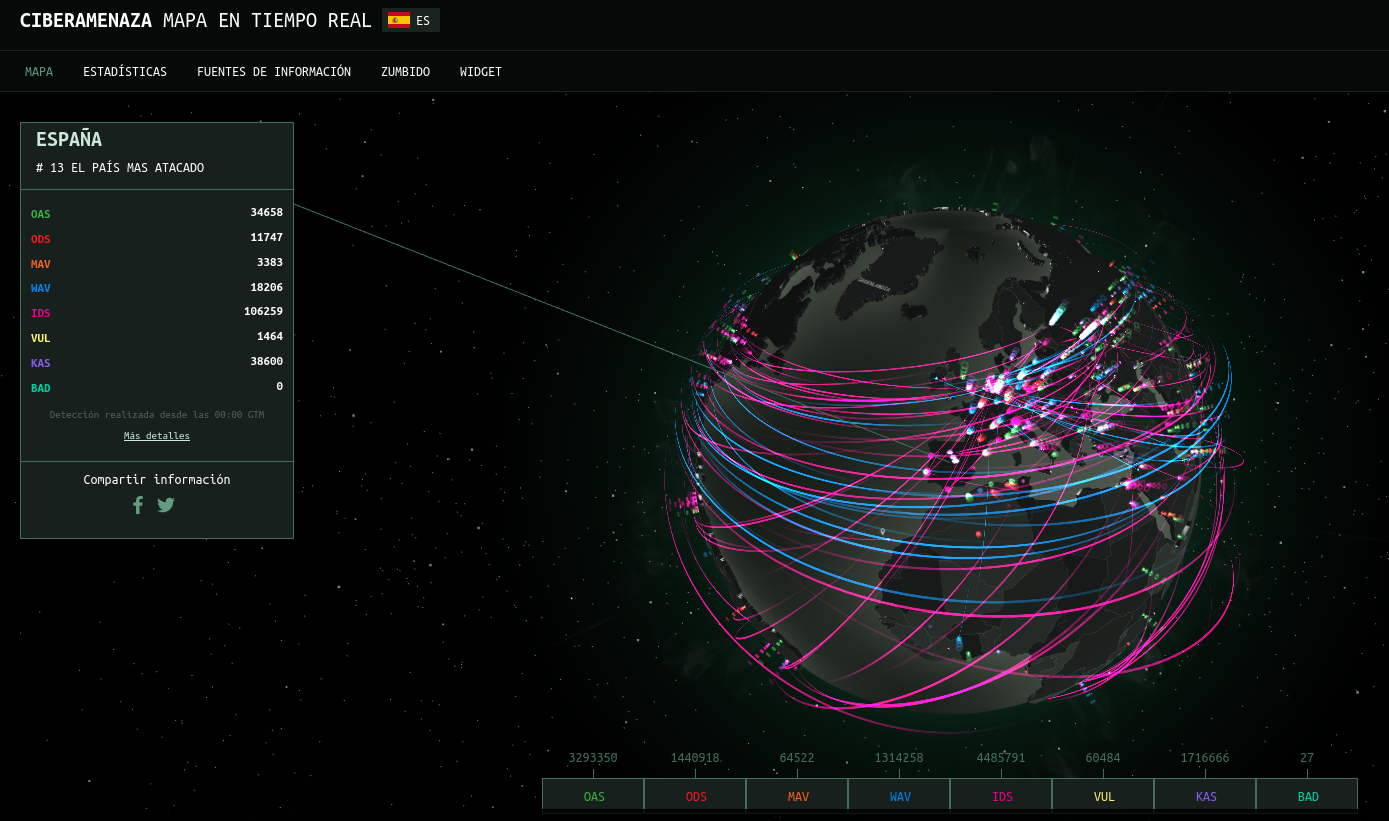
\includegraphics[scale=0.3]{imagenes/Diseno/ciberataques.png}
%		\caption[Ciberataques]{Ciberataques \cite{ciberataques:online}} 
%		\label{Ciberataques}
%	\end{figure}
%	Es por esto que se hace necesaria la protección de la infraestructura final, exponiendo únicamente los puertos necesarios para desviar el tráfico y trabajar con los servicios únicamente dentro de la red LAN segura. \\
%	Para este fin se ha elegido la tecnología pfSense \cite{pfsense:online}. PfSense dispone de su versión community gratuita y de código abierto. Esta tecnología se ha elegido ya que es la tecnología utilizada en el cluster de producción de la empresa y es un requisito.
%\end{text}
%
%\subsubsection{Contenedores}
%\begin{text}
%	Como ya hemos visto, Proxmox nos proporciona una capa de virtualización del hardware de los servidores para poder crear máquinas virtuales donde alojar los distintos servicios. \\
%	Sin embargo, a la hora del desarrollo y despliegue de aplicaciones web en el cluster, se hace inviable crear una máquina virtual por cada una de las aplicaciones web creadas. Esto sería insostenible ya que las máquinas virtuales demandan recursos. \\
%	
%	Para solventar este problema se van a crear aplicaciones en contenedores. Cada aplicación tendrá uno o varios contenedores dependiendo de los servicios, normalmente 1 servicio 1 contenedor. Para realizar este proceso se ha elegido la tecnología Docker. \cite{docker:online}.
%\end{text}
%
%\begin{text}
%	Docker es la tecnología más famosa para crear contenedores. Gracias a Docker podemos aislar las aplicaciones en contenedores seguros y fácilmente replicables. Se ha elegido Docker por su extensa comunidad y porque es la tecnología más utilizada para este fin. Sin embargo, con esto no es suficiente ya que, una vez tengamos la aplicación separada en contenedores, necesitamos un entorno donde lanzar estos contenedores y poder gestionarlos. Es aquí donde surgen los orquestadores de contenedores. A continuación se hace una pequeña a dos orquestadores: Docker Swarm \cite{swarm:online} y Kubernetes \cite{k8:online}.
%\end{text}
%
%\subsubsection{Orquestación contenedores}
%\begin{itemize}
%	\item \textbf{Docker Swarm}. Docker Swarm es un software de orquestación de contenedores. Es la solución nativa de Docker para la gestión de los contenedores. Docker Swarm nos permite automatizar los procesos de despliegue escalado y gestión de contenedores. Sin embargo, cuando hablamos de escalado vertical o horizontal, Docker Swarm, al contrario que Kubernetes, no permite este escalado asegurando la disponibilidad. Debemos relanzar los contenedores con los nuevos parámetros para el escalado. \\
%	Se ha elegido esta tecnología por ser la usada en un principio en la empresa para la gestión de contenedores. Cabe destacar que, aunque no ofrece los mismos servicios que Kubernetes, Docker Swarm es una solución muy buena para la orquestación de contenedores y su principal ventaja frente a Kubernetes es la facilidad para desplegar y gestionar los contenedores.
%	\item \textbf{Kubernetes}. Kubernetes es un software de orquestación de contenedores que nos permite automatizar el proceso de despliegue, escalado y gestión de las aplicaciones en contenedores. Kubernetes se ha convertido en la solución principal para grandes empresas por su robustez. La principal ventaja de Kubernetes frente a sus competidores es la posibilidad de modificar las condiciones de escalado vertical o horizontal de los contenedores sin afectar a la disponibilidad de la aplicación. Su gran desventaja es la complejidad, ya que para poder manejar de forma eficiente un cluster de Kubernetes debemos pasar por un largo camino de aprendizaje. \\
%	Se ha elegido esta tecnología por su gran demanda en el sector y como proceso de aprendizaje. Esta tecnología no estaba implementada en la empresa, sin embargo, se va a introducir como orquestador adicional.
%\end{itemize}
%
%\subsubsection{Almacenamiento estático}
%\label{ceph}
%\begin{text}
%	Si bien tanto Docker Swarm como Kubernetes nos permiten gestionar los contenedores, estas tecnologías están pensadas para aplicaciones stateless o sin estado \cite{stateless:online}. A grandes rasgos, esto quiere decir que tanto Kubernetes como Docker Swarm, funcionan bien con aplicaciones que no necesitan almacenar información para su correcto funcionamiento. \\
%	Para esto, Docker ofrece una solución en forma de volúmenes. Sin embargo, esta solución no se adecua a las necesidades de un entorno de alta disponibilidad  y alta fiabilidad. Es por esto que surge la necesidad de crear alguna solución de almacenamiento distribuido que nos proporcione dichas características. La solución elegida ha sido Ceph \cite{ceph:online}. Una vez más el uso de Ceph es un requisito impuesto por la empresa.
%\end{text}
%	
%\subsubsection{Servidor Web / Proxy}
%\begin{text}
%	Para el correcto acceso de los clientes y desarrolladores a las aplicaciones, se hace necesario un proxy que desvíe las peticiones a la aplicación correcta. Para este fin se ha elegido la tecnología Nginx \cite{nginx:online}, que sirve a la vez de servidor web y de proxy. Un proxy es esencial para asegurar la seguridad del cluster, ya que únicamente hay un punto de entrada protegido por un proxy que a su vez está protegido por el firewall. De esta forma se aumenta la seguridad y se dificultan los intentos de ataque masivos. Se ha elegido Nginx por ser el usado en la empresa. Forma parte de los requisitos del proyecto impuestos por la empresa.
%\end{text}
%
%\subsubsection{Control de versiones}
%\label{gitlab}
%\begin{text}
%	Para el correcto desarrollo del software y en este caso de la infraestructura, es necesario disponer de un servicio de control de versiones donde subir el código y llevar un seguimiento del mismo. Esto es muy importante, ya que cualquier cambio en el código queda reflejado y hacer rollbacks a versiones anteriores es posible. Para este fin se ha elegido la herramienta basada en git GitLab \cite{gitlab:online}. La elección de esta herramienta satisface los requisitos impuestos por la empresa.
%\end{text}
%
%
%\subsubsection{Base de datos}
%\begin{text}
%	Las aplicaciones lanzadas tanto en Docker Swarm como en Kubernetes, necesitarán almacenar el estado de la aplicación así como datos necesarios para el correcto funcionamiento de esta. Estos datos deben ser persistentes y no borrarse ante el reinicio de los contenedores o re-despliegue. Para esto, es necesario tener una base de datos que nos proporcione almacenamiento para las aplicaciones. La tecnología elegida para esta causa ha sido MariaDB, ya que las aplicaciones necesitan bases de datos relacionales y MariaDB está licenciado por GNU General Public License, así que lo podemos usar sin problemas. También se ha elegido esta tecnología porque es con la que más familiarizados estamos todos en la empresa. \\
%	Para garantizar la alta disponibilidad y alto rendimiento a la hora de recuperar datos, se ha optado por la creación de un cluster de Galera \cite{galeracluster:online} con 3 nodos, uno en cada nodo principal de Proxmox. El uso de Galera forma parte de los requisitos impuestos por la empresa.
%\end{text}

\section{Diseño de la solución basado en Ansible}
\begin{text}
	Como se ha discutido en la sección ``\nameref{tecnologias_elegidas}'' hemos elegido Ansible para cumplir los objetivos de este proyecto. Ansible nos permite automatizar el proceso de creación y configuración de la infraestructura. En la siguiente sección se hace un análisis de como se ha ido construyendo la solución utilizando Ansible en términos de metodología y forma de estructura el proyecto.
\end{text}

\subsection{Estructura, modularización y metodología}
\begin{text}
	Para diseñar la estructura y la metodología a seguir en el desarrollo se ha partido de los ``\nameref{requisitosfuncionales}''. Para entender la metodología utilizada hay que conocer como funciona Ansible.
	
	\subsubsection{Ansible}
	\label{ansible_}
	\begin{text}
		Ansible es una herramienta de automatización que nos permite lanzar playbooks contra servidores remotos o locales.
		\begin{itemize}
			\item \textbf{Playbooks}: un playbook consiste en un conjunto de tareas que se ejecutan de forma secuencial en los hosts definidos. Sin embargo, los playbooks por si solos aportan poca flexibilidad a la hora de estructurar los proyectos y dificulta la comprensión de estos ya que se pueden convertir en ficheros muy largos difíciles de seguir. Es por esto que surge la necesidad de organizar de algún modo las tareas por funcionalidad. Es aquí donde surgen los roles.
			
			\item \textbf{Roles:}: un role nos permite agrupar múltiples tareas bajo un mismo nombre. Por ejemplo, podríamos crear un role llamado firewall en el cual definiríamos todas las tareas que involucren al firewall. Ésto hace que el proyecto sea más legible y ayuda al futuro desarrollo.
		\end{itemize}
	
	Para cada caso de uso definido en ``\nameref{casosdeuso}'' se ha creado un playbook. En nuestro caso, hemos creado un role para cada servicio desplegado en el cluster. Estos roles harán los playbooks más legibles. \\
	En cada role se definen una serie de variables para decidir qué tareas se van a lanzar. Para explicar esto pongamos el ejemplo del role \textbf{webproxy}. Este role tiene varias tareas:
	\begin{itemize}
		\item \textbf{apply\_config.yml}
		\item \textbf{create\_site.yml}
		\item \textbf{create\_ssl\_cert.yml}
		\item \textbf{install\_certbot.yml}
		\item \textbf{install\_nginx.yml}
	\end{itemize}

	Podría darse el caso que quisieramos crear un sitio en nginx sin certificado SSL. Para esto se han definido unas variables que se han de definir en cada playbook para elegir qué tareas lanzar de cada role. \\
	Cada tarea definida en los role, corresponde con un issue definido en ``\nameref{issues}''.
	
	\clearpage
	
	A continuación se listan los distintos playbooks definidos y se relacionan con sus correspondientes ``\nameref{requisitosfuncionales}'' e ``\nameref{issues}''.
	
	\begin{itemize}
		\item \textbf{configure\_local\_environment.yml}. \hyperref[RF0]{RF0}.
		\begin{itemize}
			\item Issue 0.1 - 0.2.
		\end{itemize}
	
		\item \textbf{configure\_proxmox\_node.yml}. \hyperref[RF1]{RF1}, \hyperref[RF4]{RF4}.
		\begin{itemize}
			\item Issue 1 - 1.10.
		\end{itemize}
	
		\item \textbf{apply\_config\_pfsense.yml}. \hyperref[RF3]{RF3}, \hyperref[RF4]{RF4}.
		\begin{itemize}
			\item Issue 2.3.
		\end{itemize}
	
		\item \textbf{deploy\_pfsense\_firewall.yml}. \hyperref[RF3]{RF3}, \hyperref[RF4]{RF4}.
		\begin{itemize}
			\item Issue 2.1,2.2,2.4.
		\end{itemize}
		
		\item \textbf{create\_gitlab.yml}. \hyperref[RF3]{RF3}, \hyperref[RF4]{RF4}.
		\begin{itemize}
			\item Issue 3.1 - 3.4.
		\end{itemize}
	
		\item \textbf{create\_ceph\_cluster.yml}. \hyperref[RF3]{RF3}, \hyperref[RF4]{RF4}.
		\begin{itemize}
			\item Issue 5.1.
		\end{itemize}
	
		\item \textbf{create\_virtualmin.yml}. \hyperref[RF3]{RF3}, \hyperref[RF4]{RF4}.
		\begin{itemize}
			\item Issue 5.3.
		\end{itemize}
	
		\item \textbf{create\_webproxy.yml}. \hyperref[RF3]{RF3}, \hyperref[RF4]{RF4}.
		\begin{itemize}
			\item Issue 5.6.
		\end{itemize}
	
		\item \textbf{create\_icinga2.yml}. \hyperref[RF3]{RF3}, \hyperref[RF4]{RF4}.
		\begin{itemize}
			\item Issue 4.1 - 4.4.
		\end{itemize}
	
		\item \textbf{create\_galera\_cluster.yml}. \hyperref[RF3]{RF3}, \hyperref[RF4]{RF4}.
		\begin{itemize}
			\item Issue 5.2.
		\end{itemize}
	
		\item \textbf{create\_rabbitmq.yml}. \hyperref[RF3]{RF3}, \hyperref[RF4]{RF4}.
		\begin{itemize}
			\item Issue 5.5.
		\end{itemize}
	
		\item \textbf{create\_docker\_swarm\_cluster.yml}. \hyperref[RF3]{RF3}, \hyperref[RF4]{RF4}.
		\begin{itemize}
			\item Issue 5.7.
		\end{itemize}
		\item \textbf{create\_kubernetes\_cluster.yml}. \hyperref[RF3]{RF3}, \hyperref[RF4]{RF4}.
		\begin{itemize}
			\item Issue 5.7.
		\end{itemize}
		
	\end{itemize}

	\end{text}
\end{text}

\subsection{Despliegue solución}
\begin{text}
	Una vez diseñada e implementada la solución su despliegue consiste en ejecutar los distintos playbooks en la infraestructura objetivo. Sin embargo, antes de poder lanzar estos playbooks, hay que configurar un fichero \textbf{hosts.yml} donde definimos los hosts donde desplegar el proyecto así como la distribución de servicios en los nodos y otra información como la IP de cada servicio. \\
	Una vez realizada la configuración pertinente, el único requisito por parte de la empresa es el alquiler de 2 o más servidores (bare metal) en Hetzner \cite{hetzner:online}.
\end{text}

\subsection{Cumplimiento requisitos funcionales}
\begin{text}
	Al haber estructurado el proyecto creando un playbook o más por cada requisito funcional, y al tener cada role definidos una serie de test, si se cumple el objetivo de cada playbook, se cumplirán los requisitos funcionales. \\
	Como hemos comentado en la sección ``\nameref{ansible_}'', Ansible se encarga de ejecutar las tareas definidas en los roles y en los playbooks de forma secuencial. Cada tarea de Ansible tiene un objetivo el cual si no se cumple, se lanza una excepción en forma de error abortando la ejecución del playbook. Esta forma de funcionar nos asegura que, si un playbook de los definidos en este proyecto termina su ejecución con éxito, los issues a los que está asociado dicho playbook van a quedar resueltos.
\end{text}


\section{Diseño de la solución CI/CD}
\begin{text}
	Uno de los \hyperref[objetivos_primarios]{objetivos} principales de este proyecto es la creación de cauces rápidos y seguros para agilizar el proceso de creación de software.
	
	Para ello se ha pensado en el siguiente cauce utilizando el servicio de control de versiones elegido: \textbf{GitLab}.
	
	La idea es la siguiente:
		Un programador efectúa cambios en la aplicación y los sube al repositorio en GitLab. Se ejecuta un hook en GitLab que activa el pipeline. GitLab lanza la tarea pertinente a el runner que esté disponible. El runner construye la nueva imagen y la sube al registry. Finalmente, el servidor de aplicaciones donde está lanzada la aplicación, recibe un mensaje de actualización que fuerza a bajarse la nueva imagen de la aplicación y relanzarla.
	
	Cabe destacar que este proceso no implica ningún downtime en la aplicación gracias a estar desplegándolo en un cluster como docker swarm.
	\clearpage
	\begin{figure}[!hbt]
		\label{cauce_cicd}
		\centering
		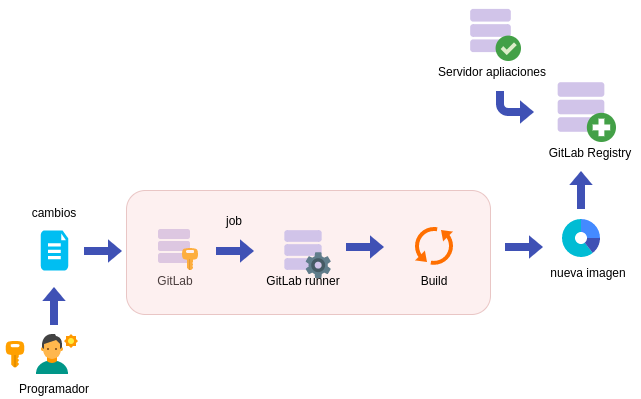
\includegraphics[scale=0.55]{imagenes/Diseno/diagrama-cicd.png}
		\caption[Cauce CI/CD]{Cauce CI/CD}
	\end{figure}
	
	Esto es posible gracias a la sección DevOps que trae GitLab incorporad que nos ofrece un registry donde almacenar las imágenes y la posiblidad de, mediante un fichero de configuración crear unas directivas para decidir qué va a ocurrir cada vez que se hace un push de una nueva versión al repositorio.
\end{text}

\section{Posibles mejoras}
        \begin{text}
            El proyecto que describe este documento, es una solución integral para resolver el problema de infraestructura en una pequeña empresa. Si hablamos de posibles mejoras, ya que siempre se puede mejorar, hablaríamos de hacer más eficientes los playbooks de Ansible o estructurarlos de forma que sean más comprensibles si cabe. Cabe destacar que en el diseño del cluster se incluye un cluster de Kubernetes, el cual está justamente para mejorar el cluster de docker-swarm. \\
            Un punto importante de mejora sería implementar las técnicas de integración continua y entrega continua a las aplicaciones Wordpress de Virtualmin, ya que en este proyecto únicamente se abordan los proyectos Django + Angular de la empresa. \\
            A grandes rasgos y exceptuando pequeñas mejoras en la calidad del código o la documentación, pienso que el proyecto es muy ambicioso y está bien diseñado a nivel de infraestructura, no necesitando grandes cambios en un futuro próximo.
        \end{text}
%
%\input{capitulos/06_Implementacion}
%
%\input{capitulos/07_Pruebas}
%
%\input{capitulos/08_Conclusiones}
%
%%\chapter{Conclusiones y Trabajos Futuros}
%
%
\nocite{*}
\bibliography{bibliografia/bibliografia}\addcontentsline{toc}{chapter}{Bibliografía}
\bibliographystyle{ieeetr}
%
%\appendix
%\input{apendices/manual_usuario/manual_usuario}
%%\input{apendices/paper/paper}
%\input{glosario/entradas_glosario}
% \addcontentsline{toc}{chapter}{Glosario}
% \printglossary
\chapter*{}
\thispagestyle{empty}

\end{document}
